\documentclass[a4paper, 10pt]{article}
%\documentclass{article}

\usepackage{stmaryrd}
\usepackage{amsfonts,amsmath,amssymb,mathtools,amsthm}
\usepackage{graphicx}
\usepackage{float}
\usepackage{blindtext}
\usepackage{enumitem}
\usepackage{xcolor}
\usepackage{thmtools}
\usepackage{tikz}
\usetikzlibrary{shapes, arrows, positioning}


\usepackage{graphicx}
%this package is flexible for image insertion
%
\usepackage{alltt}
%this package is suitable for the description of algorithms and computer programs
%
\usepackage{amsmath}
%this package draws mathematical symbols smoothly
%
\usepackage{xcolor}
\definecolor{C0}{HTML}{3182ce}
\usepackage[breaklinks=true,colorlinks,bookmarks=false,citecolor=C0]{hyperref}
\usepackage[margin=1in]{geometry}
% \usepackage[hidelinks, pdftex]{hyperref}
%this package produces hypertext links in the document
\usepackage[round]{natbib}  

\pagenumbering{arabic}
\setcounter{page}{1}
\renewcommand{\thefootnote}{\fnsymbol{footnote}}
\newcommand{\doi}[1]{\href{https://doi.org/#1}{\texttt{https://doi.org/#1}}}

\renewcommand{\P}{\mathbb{P}}
\newcommand{\E}{\mathbb{E}}
\newcommand{\arcosh}{\text{arcosh}}
\newcommand{\arsinh}{\text{arsinh}}
\newcommand{\artanh}{\text{artanh}}

\newcommand{\beq}{\begin{equation}}
\newcommand{\eeq}{\end{equation}}
\newcommand{\bea}{\begin{eqnarray}}
\newcommand{\eea}{\end{eqnarray}}
\newcommand{\beqq}{\begin{equation*}}
\newcommand{\eeqq}{\end{equation*}}
\newcommand{\beaa}{\begin{eqnarray*}}
\newcommand{\eeaa}{\end{eqnarray*}}


\newtheorem{theorem}{Theorem}[section]
\newtheorem{conjecture}{Conjecture}[section]

\newtheorem{proposition}{Proposition}[section]
\newtheorem{lemma}{Lemma}[section]
\newtheorem{corollary}{Corollary}[section]

\theoremstyle{definition}
\newtheorem{remark}{Remark}[section]
\newtheorem{definition}{Definition}[section]
\def\br{\begin{remark}\rm\small}
\def\er{\end{remark}}
\def\bt{\begin{theorem}}
\def\et{\end{theorem}}
\def\bd{\begin{definition}}
\def\ed{\end{definition}}
\def\bp{\begin{proposition}}
\def\ep{\end{proposition}}
\def\bl{\begin{lemma}}
\def\el{\end{lemma}}
\def\bc{\begin{corollary}}
\def\ec{\end{corollary}}
\def\beaq{\begin{eqnarray}}
\def\eeaq{\end{eqnarray}}


\title{Characterisation of optimal sub-Gaussian variance proxy and application to discrete distributions}
\date{}

\begin{document}

\maketitle

% \small
% \textbf {Firstname Lastname, Firstname2 Lastname2, Firstname3 Lastname3}\\[6pt]
% Institution(s) of author(s), address(es) \\ author@somewhere.host\\[6pt]
% Received: date\quad/\quad
% Revised: date\quad/\quad
% Publised online: data

\begin{abstract}
to be filled 

\end{abstract}


\section{Introduction}\label{s:1}
The sub-Gaussian property, first characterized by \citet{Kahane1960PropritsLD} and \citet{buldygin1980sub}, has become a critical tool for understanding the tail behavior of random variables. Since the pioneering work of \citet{buldygin1980sub}, this property has emerged as a fundamental concept in probability theory due to its profound implications in various mathematical disciplines, such as concentration inequalities \citep{Hoeffding1963, boucheron2003concentration, raginsky2013concentration} and Bayesian statistics \citep{elder2016bayesian, catoni2007pac, vladimirova2019understanding, vladimirova2020sub}. In machine learning, sub-Gaussian tails play a crucial role in bandit algorithms \citep{bubeck2012regret} and in the study of the singular values of random matrices \citep{rudelson2010non}.

Although extensive research has focused on continuous distributions such as Beta, Dirichlet, and multimodal distributions \citep{marchal2017sub}, as well as Bernoulli, binomial, Kumaraswamy, and triangular distributions \citep{arbel2020strict}, and truncated Gaussian and exponential distributions \citep{barreto2024optimal}, the sub-Gaussianity of discrete distributions remains underexplored, despite their prevalence in modeling count data, binary outcomes, and combinatorial stochastic processes.\\


\textbf{Definition 1 (Sub-Gaussian Variables)} A random variable \( X \) with finite mean \( \mu = \mathbb{E}[X] \) is \textit{sub-Gaussian} if there exists a constant \( \sigma^2 > 0 \) such that:
\begin{equation}
    \mathbb{E}[\exp(\lambda (X - \mu))] \leq \exp\left(\frac{\lambda^2 \sigma^2}{2}\right), \text{ for all } \lambda \in \mathbb{R}.
    \label{eq:def_sub}
\end{equation}

Such a constant \( \sigma^2 \) is called a \textit{proxy variance} (or \textit{sub-Gaussian norm}), and we say that \( X \) is \(\sigma^2\)-sub-Gaussian. When \( X \) is sub-Gaussian, the primary focus is often on determining the \textit{optimal proxy variance}:
\[
\sigma^2_{\mathrm{opt}}(X) = \inf \left\{ \sigma^2 > 0 \text{ such that } X \text{ is } \sigma^2\text{-sub-Gaussian} \right\}.
\]

For a \(\sigma^2\) sub-Gaussian random variable \(X\), the true variance is always bounded by the proxy variance, i.e. $\text{Var}(X) \leq \sigma^2$, as shown by comparing Taylor expansions of the moment-generating function. When $\sigma^2_{\mathrm{opt}}(X) = \mathrm{Var}(X)$, \(X\) is called \textit{strictly} sub-Gaussian.

\paragraph{Contributions.}

\paragraph{Outline.}

\section{Characterization of optimal sub-Gaussian variance proxy}\label{sec:charac}
Let $M_Y(\lambda):=\ln \left(\mathbb{E}[\exp(\lambda (Y - \mu))]\right)$ and define
\beq g_Y(\lambda;\sigma^2):=\frac{1}{2}\lambda^2\sigma^2- M_Y(\lambda)= \frac{1}{2}\lambda^2\sigma^2-\ln \left(\mathbb{E}[\exp(\lambda (Y - \mu))]\right)\eeq
which is a smooth function of $(\lambda,\sigma^2)$.
We have
\beq g'_Y(\lambda;\sigma^2):= \lambda\sigma^2- M_Y'(\lambda)\eeq
Observe that $g_Y(0,\sigma^2)=0=g_Y'(0,\sigma^2)$. Moreover, for $\lambda\neq 0$, the equation $g_Y'(\lambda,\sigma^2)=0$ is equivalent to $\sigma^2=\frac{M_Y'(\lambda)}{\lambda} $. Thus, the system of equations $g_Y(\lambda;\sigma^2)=0$ and $g_Y'(\lambda,\sigma^2)=0$ with $\lambda\neq 0$ is equivalent to  
\beq \sigma^2=\frac{1}{\lambda} M_Y'(\lambda) \text{ and } \lambda\neq 0 \text{ sol. of  } \lambda M_Y'(\lambda)- 2M_Y(\lambda)=0\eeq

Let us define
\beq \mathcal{L}_c^*:=\left\{\lambda_c \in \mathbb{R}^* \,/\,  \lambda_c M_Y'(\lambda_c)- 2M_Y(\lambda_c)=0 \,\, \text{ and }\lambda_c \text{ local min. of } g\left(.,\sigma^2=\frac{ M_Y'(\lambda_c)}{\lambda_c}\right) \right\}\eeq
and define 
\beq \mathcal{S}_c^*=\left\{\frac{M_Y'(\lambda_c)}{\lambda_c}  \,/\, \lambda_c\in \mathcal{L}_c\right\}\eeq
We complement them by defining:
\beq \mathcal{L}_c=\mathcal{L}_c^*\cup\{0\}\,\,, \,\mathcal{S}_c=\mathcal{S}_c^*\cup\{\text{Var}[Y]\}\eeq 

Let us first make the following observation.
\begin{proposition}[Asymptotics at infinity]\label{AsymptInf}If $M_Y(\lambda)\overset{\lambda\to\pm \infty}{=}o(\lambda^2)$ then
\beq \lim_{\lambda\to \pm\infty}g_Y(\lambda;\sigma^2)=+\infty\,,\, \lim_{\lambda\to \pm\infty}g'_Y(\lambda;\sigma^2)=\pm\infty\,,\, \lim_{\lambda\to \pm\infty}g''_Y(\lambda;\sigma^2)=\sigma^2\eeq
and $Y$ is Sub-Gaussian. Moreover a sufficient condition is that $Y$ is a bounded random variable.    
\end{proposition}

\begin{proof}The proof is obvious from the definition of $g_Y(\lambda;\sigma^2)=\frac{1}{2}\lambda^2\sigma^2-M_Y(\lambda)$. The sufficient condition is also immediate since if $M$ is a bound for $Y$ then
$|M_Y(\lambda)|\leq \lambda|M+\mu|=o(\lambda^2)$. The fact that $Y$ is Sub-Gaussian follows from the fact that there exists $C>0$ such that $|M(\lambda)|\leq C\lambda^2$ for all $\lambda\in \mathbb{R}$. Thus, taking $\sigma^2>C$ immediately gives that $\sigma^2$ is a variance proxy so that $Y$ is Sub-Gaussian.
\end{proof}

First, let us prove the following lemma.

\begin{lemma}\label{LemmaTechnicalGeneral}Assume that $M_Y(\lambda)\overset{\lambda\to \pm\infty}{=}o(\lambda^2)$. If $\sigma_{\text{opt}}^2>\text{Var}[Y]$ then $\sigma_{\text{opt}}^2$ may only be achieved when $g_Y(.;\sigma_{\text{opt}}^2)$ has at least one point $\lambda_0\in \mathbb{R}^*$ where $g(\lambda_0;\sigma_{\text{opt}}^2)=0=g_Y'(\lambda_0;\sigma_{\text{opt}}^2)$. In other words, $\lambda_0\in \mathcal{L}_c^*$ and $\sigma_{\text{opt}}^2=\frac{M_Y'(\lambda_0)}{\lambda_0}\in \mathcal{S}_c^*$.
\end{lemma}

\begin{proof}First, \autoref{AsymptInf} provides control at infinity of the function $g_Y(.;\sigma^2)$ which is positive and locally convex at $\pm \infty$. Then, let us define $\sigma_0^2=\sigma_{\text{opt}}^2 -\frac{1}{2}(\sigma_{\text{opt}}^2-\text{Var}[Y])$. Then observe that for any $\sigma^2\in \left(\sigma_0^2,\sigma_{\text{opt}}^2\right)$, $g(.;\sigma^2)$ is convex non-negative around $\lambda=0$ with $g''(0,\sigma^2)>\sigma_0^2-\text{Var}[Y]>0$. In particular, there exists an interval $(-a,a)$ with $a>0$ where $(\lambda,\sigma^2)\mapsto g(\lambda;\sigma^2)$ is locally positive for any $\lambda\in (-a,a)\setminus\{0\}$ and any $\sigma^2\in \left(\sigma_0^2,\sigma_{\text{opt}}^2\right)$ and such that there exists $A>0$ such that $\underset{\sigma\in \left(\sigma_0^2,\sigma_{\text{opt}}^2\right)}{\text{Sup}}\left\{g(-a;\sigma^2),g(a;\sigma^2)\right\}>A$. Thus, for any $\sigma^2\in \left(\sigma_0^2,\sigma_{\text{opt}}^2\right)$, $g(.;\sigma^2)$ has no local minimum except $0$ in $(-a,a)$. Let us consider a local minimum $\lambda_m\neq 0$ (i.e. $|\lambda_m|\geq a$ from the previous discussion) of $g(.;\sigma_{\text{opt}}^2)$ and define $M_m=g(\lambda_m;\sigma_{\text{opt}}^2)$. It is obvious that $M_m$ cannot be strictly negative, otherwise by continuity of $\sigma\to g(\lambda_m;\sigma^2)$, there would exist $\epsilon>0$ such that for any $\sigma^2\in \left(\sigma_{\text{opt}}^2, \sigma_{\text{opt}}^2+\epsilon\right)$: $g(\lambda_m,\sigma^2)<0$ so that $\sigma^2$ would not be a proxy variance in contradiction with the fact that $\sigma_{\text{opt}}^2$ is the optimal variance proxy. Thus we must have $M_m\geq 0$. Assume now by contradiction that there exists $\eta>0$ such that we have all $M_m>\eta$ for all local minima. We shall take $\eta$ sufficiently small so that $\eta<\frac{A}{3}$. In particular, we get that the global minimum of $g(.;\sigma_{\text{opt}}^2)$ on $(-\infty,-a)\cup(a,+\infty)$ is greater than $\eta$. Since $\underset{\lambda\to \pm \infty}{\lim} g(\lambda;\sigma^2)=+\infty$, we may use continuity on a compact set to prove that there exists $\epsilon>0$, with $\epsilon<\frac{1}{2}(\sigma_{\text{opt}}^2-\text{Var}[Y])$ such that the global minimum of $g(.;\sigma^2)$ is greater than $\frac{\eta}{2}$ for any $\sigma^2\in \left(\sigma_{\text{opt}}^2-\epsilon,\sigma_{\text{opt}}^2\right)$. In other words, we may lower $\sigma^2$ from $\sigma_{\text{opt}}^2$ while $g(.;\sigma^2)$ remains non-negative and hence is a proxy variance. This contradicts the fact that $\sigma_{\text{opt}}^2$ is optimal and ends the proof of \autoref{LemmaTechnicalGeneral}.  
\end{proof} 


The optimal proxy variance is characterized by the following theorem.

\begin{theorem}[Characterization of the optimal variance proxy]\label{GeneralCharac} Let us assume that $M_Y(\lambda)\overset{\lambda\to \pm\infty}{=}o(\lambda^2)$. Then, the optimal proxy variance is characterized by
\beq \sigma_{\text{opt}}^2=\text{Max}\left\{\text{Var}[Y],\underset{s\in \mathcal{S}_c^*}{\text{Sup}}(s)\right\}\eeq    
\end{theorem}

\begin{proof}Let us first consider $\sigma^2>\text{Max}\{\text{Var}[Y],\text{Sup}_{s\in \mathcal{S}_c^*}(s)\}$. Then since $\sigma^2>\text{Var}[Y]$, we get that $g(.;\sigma^2)$ is locally convex and non-negative around $\lambda=0$.  Let us consider $\lambda_m(\sigma)\neq 0$ a local minimum of $g(.,\sigma^2)$. For simplicity we shall assume that $\lambda_m(\sigma)>0$ but a similar argument is valid if $\lambda_m(\sigma)<0$. Then we have $\partial_{\sigma}[g(\lambda_m(\sigma);\sigma^2)]= g'(\lambda_m(\sigma);\sigma^2) \partial_\sigma \lambda_m(\sigma) + \lambda_m(\sigma)^2\sigma= \lambda_m(\sigma)^2\sigma>0$. Assume by contradiction that $g(\lambda_m(\sigma);\sigma^2)<0$ then increasing $\sigma$ would increase the value of $g(\lambda_m(\sigma);\sigma^2)$. Since $\partial_{\sigma}[g(\lambda_m(\sigma);\sigma^2)]=\lambda_m(\sigma)^2\sigma>0$ there are only two cases: \begin{itemize}\item $\lambda_m(\sigma)$ remains outside a positive neighborhood of $0$ denoted $(0,\epsilon)$ when we increase $\sigma$ and thus since $\partial_{\sigma}[g(\lambda_m(\sigma);\sigma^2)]>\epsilon^2 \sigma$ there exists a value $\sigma_1>\sigma$ for which $g(\lambda_m(\sigma_1);\sigma_1^2)=0$ which is a contradiction because $\sigma_1^2\in \mathcal{S}_c^*$ so that we should have $\sigma\geq \sigma_1$.
\item $\lambda_m(\sigma)\to 0_+$ when we increase $\sigma$. In this case this is a contradiction because $g(.,\sigma^2)$ is locally positive and convex in a positive neighborhood of $0$. Indeed, $g(.,\sigma^2)$ must reach a positive local maximum on $(0,\lambda_m(\sigma))$ that we denote $\lambda_{\text{max}}(\sigma)$. By Rolle's theorem on $(0,\lambda_{\text{max}}(\sigma))$ and $(\lambda_{\text{max}}(\sigma),\lambda_m(\sigma))$, there exist at least two distinct values $(\lambda_1(\sigma),\lambda_2(\sigma))$ with $0<\lambda_1(\sigma)<\lambda_{\text{max}}(\sigma)<\lambda_2(\sigma)<\lambda_m(\sigma)$ such that $g''(\lambda_1(\sigma);\sigma^2)=g''(\lambda_2(\sigma);\sigma^2)=0$. Since $\lambda_m(\sigma)\to 0_+$, we must also have $\lambda_1(\sigma),\lambda_2(\sigma)\to 0_+$ and hence by continuity $g''(0,\sigma^2)\to 0$. But this is impossible since $g''(0;\sigma^2)=(\sigma^2-\text{Var}[Y])>0$ is a positive, increasing function of $\sigma$. 
\end{itemize}
Thus we conclude that for any $\sigma^2>\text{Max}\{\text{Var}[Y],\text{Sup}_{s\in \mathcal{S}_c^*}(s)\}$, all local minima of $g(.;\sigma^2)$ are non-negative so that since $\underset{\lambda\to \pm \infty}{\lim} g(\lambda;\sigma^2)=+\infty$, $g(.;\sigma^2)$ is non-negative on $\mathbb{R}$. Hence $\sigma^2$ is a variance proxy and thus $\sigma_{\text{opt}}^2\leq \text{Max}\{\text{Var}[Y],\text{Sup}_{s\in \mathcal{S}_c^*}(s)\}$.

\medskip

\sloppy{Let us prove the converse inequality and assume that $\sigma_{\text{opt}}^2< \text{Max}\{\text{Var}[Y],\text{Sup}_{s\in \mathcal{S}_c^*}(s)\}$. It is well-known that $\text{Var}[Y]$ is always a lower bound for the optimal proxy variance, thus the last inequality is only possible if  $\text{Var}[Y]<\sigma_{\text{opt}}^2< \text{Sup}_{s\in \mathcal{S}_c^*}(s)$.} Thus, there exists $s_c\in \mathcal{S}_c^*$ such that $\sigma_{\text{opt}}^2<s_c$, i.e. there exists $\lambda_c\in \mathbb{R}^*$ such that $g(\lambda_c;s_c)=g'(\lambda_c;s_c)=0$ and $\lambda_c$ is a local minimum of $g(.;s_c)$. We have from the fact that the dependence of $g$ relatively to $\sigma$ is quadratic that:
\beq g(\lambda_c,\sigma^2)=g(\lambda_c,s_c) +\frac{1}{2}\lambda_c^2 (\sigma^2-s_c)=\frac{1}{2}\lambda_c^2 (\sigma^2-s_c)\eeq
so that $g(\lambda_c,\sigma^2)<0$ when $\sigma^2<s_c$. This implies that $g(.;\sigma^2)$ is no longer non-negative when $\sigma^2<s_c$ so that $\sigma^2$ is not a proxy variance. This contradicts the fact that $\sigma_{\text{opt}}^2<s_c$ is an optimal proxy variance.
\end{proof}


\begin{remark}The main advantage of the characterization of the optimal proxy variance by \autoref{GeneralCharac} is that it gives a numeric way to obtain the optimal proxy variance in practice. Indeed, in order to determine it, one can numerically solve for the equation $\lambda M'(\lambda)-2M(\lambda)=0$. When numeric solutions are found, one should check numerically if $\lambda$ is a local minimum of $g\left(.;\sigma^2=\frac{M'(\lambda)}{\lambda}\right)$ (a sufficient condition being that $g''\left(\lambda;\sigma^2=\frac{M'(\lambda)}{\lambda}\right)>0$). Collecting all solutions, one picks the optimal proxy variance by looking at the maximal values of $\frac{M'(\lambda)}{\lambda}$ that can easily be computed numerically. In practice, such an algorithm is particularly efficient if the number of solutions of $\lambda M'(\lambda)-2M(\lambda)=0$ is low and if one can bound the intervals on which to look for numeric solutions.  
\end{remark}

\textcolor{blue}{In practice, for a given family of distributions, one should study the cardinal of $\mathcal{L}_c^*$ and if any compare the corresponding values of $s_c$ to select the optimal variance proxy.}


\textcolor{orange}{In our case, there are only one non-zero solution when $p_3<4\sqrt{p_1p_2}$ and it is explicit: $2\lambda_0$. In the second regime, we have two non-zero solutions: $2\lambda_0$ and another one on $\mathbb{R}_+$ and we should compare their corresponding values of $s_c$ to decide which gives the optimal variance proxy.}

Another useful result in practice is given in the following general lemma. 

\begin{lemma}\label{LemmaNumber}[Local minimum when $g_Y''(.;\sigma^2)$ has two positive zeros and $\sigma^2>\text{Var}[Y]$]
Assume that $M_Y(\lambda)\overset{\lambda\to \pm\infty}{=}o(\lambda^2)$ and that for any $\sigma^2\in \left(\text{Var}[Y],+\infty\right)$, $g''(.;\sigma^2)$ has exactly two zeros $(\lambda_1(\sigma),\lambda_2(\sigma))$ such that $0<\lambda_1(\sigma)<\lambda_2(\sigma)$. Then, $g(.;\sigma^2)$ has at most one local minimum on $\mathbb{R}_+^*$. More precisely, if there exists $\sigma_1^2\in \left(\text{Var}[Y],\sigma_0^2\right)$ such that $g'(.;\sigma_1^2)$ has a zero on $\mathbb{R}_+^*$, then  $g(.;\sigma^2)$ is strictly positive for $\sigma^2\geq\sigma_1^2$ and $g(.;\sigma^2)$ admits a unique local minimum $\lambda_m(\sigma)$ on $\mathbb{R}_+^*$ located in $\lambda_m(\sigma)\in\left(\lambda_1(\sigma),\lambda_2(\sigma)\right)$ for $\text{Var}[Y]<\sigma^2<\sigma_1^2$. Finally $\lambda_m(\sigma)$ is a increasing function of $\sigma$, so that:
\begin{itemize}
    \item The equations $g(\lambda,\sigma^2)=0=g'(\lambda,\sigma^2)$ has at most one solution on $(\lambda,\sigma^2)\in \mathbb{R}_+^*\times \left(\text{Var}[Y],+\infty\right)$.
    \item If the equations $g(\lambda,\sigma^2)=0=g'(\lambda,\sigma^2)$ has no solution on $\mathbb{R}_+^*\times \left(\text{Var}[Y],+\infty\right)$ then, $g(.;\sigma^2)$ is non-negative on $\mathbb{R}_+$ for any $\sigma^2>\text{Var}[Y]$.
    \item If the equations $g(\lambda,\sigma^2)=0=g'(\lambda,\sigma^2)$ has a solution $(\lambda_c,\sigma_c^2)\in \mathbb{R}_+^*\times \left(\text{Var}[Y],+\infty\right)$, then it is necessarily a local minimum and $g(.;\sigma^2)$ is non-negative on $\mathbb{R}_+$ if and only if $\sigma^2\geq \sigma_c^2$. 
\end{itemize}
A similar result is valid on $\mathbb{R}_-^*$. 
\end{lemma}

\begin{proof}The proof follows from the study of variations. Indeed, let us first notice that for any $\sigma^2>\text{Var}[Y]$, we have that $g(.;\sigma^2)$ is locally convex and positive around $\lambda=0$ since $g''(0;\sigma^2)=\sigma^2-\text{Var}[Y]>0$. We also remind that $\underset{\lambda\to \pm \infty}{\lim} g''(\lambda;\sigma^2)=\sigma^2>0$. so that $g(.;\sigma^2)$ is also convex at infinity. Thus, from the assumption that $g''(.;\sigma^2)$ has exactly two zeros $(\lambda_1(\sigma),\lambda_2(\sigma))$ on $\mathbb{R}_+^*$, we conclude either $g''(.;\sigma^2)$ does not change sign at its zeros and in this case, $g(.;\sigma^2)$ is strictly convex on $\mathbb{R}_+^*$ with $g(0;\sigma^2)=0$ so that it is positive and increasing on $\mathbb{R}_+$, thus there is no solution of $g'(.;\sigma^2)=0$ on $\mathbb{R}_+^*$. Or that $g''(.;\sigma^2)$ is necessarily positive on $(0,\lambda_1(\sigma))$, negative on $(\lambda_1(\sigma),\lambda_2(\sigma))$ and positive on $(\lambda_2(\sigma),+\infty)$. Thus, $g'(.;\sigma^2)$ is increasing on $(0,\lambda_1(\sigma))$ and since $g'(0;\sigma^2)$ it is positive on $(0,\lambda_1(\sigma))$. Then, $g'(.;\sigma^2)$ is decreasing on $(\lambda_1(\sigma),\lambda_2(\sigma))$ and then increasing on $(\lambda_2(\sigma),+\infty)$. In particular $g'(.;\sigma^2)$ admits a unique local minimum at $\lambda=\lambda_2(\sigma)$ on $\mathbb{R}_+^*$. Consequently, if $g'(\lambda_2(\sigma);\sigma^2)\geq 0$, then $g(.;\sigma^2)$ is non-negative on $\mathbb{R}_+$ and thus since $g(0;\sigma^2)=0$, we get that $g(.;\sigma^2)$ is non-negative on $\mathbb{R}_+$. Alternatively, if $g'(\lambda_2(\sigma);\sigma^2)<0$, then $g'(.;\sigma^2)$ has exactly two zeros $\lambda_1(\sigma)<\lambda_l(\sigma)<\lambda_r(\sigma)<\lambda_2(\sigma)$ and it is negative on $(\lambda_l(\sigma),\lambda_r(\sigma))$ and positive on $(0,\lambda_l(\sigma))\cup(\lambda_r(\sigma),+\infty)$. Consequently, $g(.;\sigma^2)$ has exactly one local minimum on $\mathbb{R}_+^*$ which is necessarily located in  $(\lambda_1(\sigma),\lambda_2(\sigma))$.
Next, let us observe that:
\beq \partial_\sigma[g'(\lambda_2(\sigma);\sigma^2)]=g''(\lambda_2(\sigma);\sigma^2) \partial_\sigma[\lambda_2(\sigma)]+ 2\sigma\lambda_2(\sigma)=2\sigma\lambda_2(\sigma)>0\eeq
Thus, the local minimum of $g'(.;\sigma^2)$ is an increasing function of $\sigma$, so that if it is null for a value $\sigma_1$, then it is positive for $\sigma>\sigma_1$ and negative for $\sigma<\sigma_1$.
Finally, let us observe that
\beq  \partial_\sigma[g(\lambda_m(\sigma);\sigma^2)]=g'(\lambda_m(\sigma);\sigma^2) \partial_\sigma[\lambda_m(\sigma)]+ \sigma\lambda_m(\sigma)^2=\sigma\lambda_m(\sigma)^2>0\eeq
so that $\lambda_m(\sigma)$ is a increasing function of $\sigma$. Let us denote $(\lambda_c,\sigma_c^2)\in \mathbb{R}_+^*\times \left(\text{Var}[Y],+\infty\right)$ a solution of $g(\lambda,\sigma^2)=0=g'(\lambda,\sigma^2)$, then for $\sigma<\sigma_c$, we have $g(\lambda_m(\sigma);\sigma^2)<0$ while for $\sigma>\sigma_c$, we have $g(\lambda_m(\sigma);\sigma^2)>0$. Since $g(.;\sigma^2)$ has only a unique local minimum $\lambda_m(\sigma)$ and a local maximum on $\mathbb{R}_+^*$ which is always strictly positive, we conclude that we cannot have another solution of $g(\lambda,\sigma^2)=0=g'(\lambda,\sigma^2)$ with $\lambda\in \mathbb{R}_+^*$. When there is no solution, we have $g(\lambda_m(\sigma);\sigma^2)>0$ so that $g(.;\sigma^2)$ is non-negative on $\mathbb{R}_+^*$. When we have a unique solution $(\lambda_c,\sigma_c^2)$, then $g(\lambda_m(\sigma);\sigma^2)>0$ for $\sigma>\sigma_c$, $g(\lambda_m(\sigma_c);\sigma_c^2)=0$ and $g(\lambda_m(\sigma);\sigma^2)<0$ for $\sigma<\sigma_c$ concluding the proof. 
\end{proof}

\begin{remark} The cases where $g''$ has no or one zero on $\mathbb{R}_+^*$ are trivial for $\sigma^2\geq \text{Var}[Y]$. Indeed, if $g''(.;\sigma^2)$ has no zero on $\mathbb{R}_+^*$, then it is strictly convex on $\mathbb{R}_+^*$ and since $g(0;\sigma^2)=g'(0;\sigma^2)=0$, $g(.;\sigma^2)$ is positive on $\mathbb{R}_+^*$. If $g''(.;\sigma^2)$ has a unique zero on $\mathbb{R}_+^*$, then it cannot change sign at this zero, because $g''(0;\sigma^2)=\sigma^2-\text{Var}[Y]\geq 0$ and $\underset{\lambda\to +\infty}{\lim}g''(\lambda;\sigma^2)=\sigma^2>0$. Hence, we conclude similarly that $g(.;\sigma^2)$ is positive on $\mathbb{R}_+^*$. 
\end{remark}

We may complement \autoref{LemmaNumber} with another lemma regarding the situation when $\sigma<\sigma_{\text{opt}}$.

\begin{lemma}\label{LemmaNumber2}[Local minimum when $g_Y''(.;\sigma^2)$ has two positive zeros and $\sigma^2<\text{Var}[Y]$]
Assume that $M_Y(\lambda)\overset{\lambda\to \pm\infty}{=}o(\lambda^2)$ and that for any $\sigma^2\in \left(0,\text{Var}[Y]\right)$, $g''(.;\sigma^2)$ has exactly two zeros $(\lambda_1(\sigma),\lambda_2(\sigma))$ such that $0<\lambda_1(\sigma)<\lambda_2(\sigma)$. Then, there is no solution to the set of equations $g_Y(\lambda;\sigma^2)=0=g_Y'(\lambda;\sigma^2)$ with $\lambda>0$ and $\sigma^2\in \left(0,\text{Var}[Y]\right)$.\\
A similar result holds on $\mathbb{R}_-^*$.
\end{lemma}

\begin{proof}For any $\sigma^2<\text{Var}[Y]$, we have that $g_Y(\lambda\sigma^2)=(\sigma^2-\text{Var}[Y])\lambda^2+o(\lambda^2)$ when $\lambda\to 0_+$. Thus, $g(.;\sigma^2)$ is locally concave and negative around $\lambda=0_+$. Since  $M_Y(\lambda)\overset{\lambda\to \pm\infty}{=}o(\lambda^2)$, we know that $g_Y(.;\sigma^2)$ is locally convex and positive when $\lambda\to +\infty$. Since $g_Y''(.;\sigma^2)$ is assumed to have exactly two positive zeros $\lambda_1(\sigma)<\lambda_2(\sigma)$, we may only have the following cases:
\begin{itemize}
    \item $g''_Y(.;\sigma^2)$ is negative on $(0,\lambda_1(\sigma))$ and changes sign at $\lambda_1(\sigma)$. Thus, it is positive on $(\lambda_1(\sigma),\lambda_2(\sigma))$ and cannot change sign at $\lambda_2(\sigma)$ to remain positive at $+\infty$. Hence, $g''_Y(.;\sigma^2)$ is positive on $(\lambda_1(\sigma),\lambda_2(\sigma))\cup (\lambda_2(\sigma),+\infty)$. Consequently, $g'_Y(.;\sigma^2)$ is decreasing on $(0,\lambda_1(\sigma))$ and increasing on $(\lambda_1(\sigma),+\infty)$. Since $g'_Y(0;\sigma^2)$, we have $g'_Y(\lambda_1(\sigma);\sigma^2)<0$ and since $g'_Y(+\infty;\sigma^2)=+\infty$, $g'_Y$ has only one zero $\lambda_0(\sigma)$ on $\mathbb{R}_+^*$ that satisfies $\lambda_0(\sigma)>\lambda_1(\sigma)$. Moreover, $g'_Y(.;\sigma^2)$ is negative on $(0,\lambda_0(\sigma))$ and positive on $(\lambda_0(\sigma),+\infty)$. Hence, $g_Y(.;\sigma^2)$ is decreasing on $(0,\lambda_0(\sigma))$ and increasing on $(\lambda_1(\sigma),+\infty)$. Since $g_Y(0;\sigma^2)=0$ and $g_Y(+\infty;\sigma^2)=+\infty$, $g_Y$ admits a unique zero $\lambda_*(\sigma)$ on $\mathbb{R}_+^*$ and we have $\lambda_*(\sigma)>\lambda_0(\sigma)$. Hence, there are no simultaneous solutions to $g_Y(\lambda;\sigma^2)=0=g_Y'(\lambda;\sigma^2)$ with $\lambda>0$.
    \item $g''_Y(.;\sigma^2)$ is negative on $(0,\lambda_1(\sigma))$ and does not change sign at $\lambda_1(\sigma)$ so it is negative on $(0,\lambda_2(\sigma))$. In order to be positive at $\lambda\to +\infty$, $g_Y''(.;\sigma^2)$ must change sign at $\lambda=\lambda_2(\sigma)$. Thus, $g_Y'(.;\sigma^2)$ is decreasing on $(0,\lambda_2(\sigma))$ and increasing on $(\lambda_2(\sigma),+\infty)$. Since $g_Y'(0;\sigma^2)=0$ and $g_Y'(+\infty;\sigma^2)=+\infty$, $g_Y'(.;\sigma^2)$ admits a unique zero $\lambda_0(\sigma)$ on $\mathbb{R}_+^*$ and it satisfies $\lambda_0(\sigma)>\lambda_2(\sigma)$. Moreover, $g_Y'(.;\sigma^2)$ is negative on $(0,\lambda_0(\sigma))$ and positive on $(\lambda_0(\sigma),+\infty)$. Since $g_Y(0;\sigma^2)=0$ and $g_Y(+\infty;\sigma^2)=+\infty$, $g_Y(.,\sigma^2)$ is decreasing and negative on $(0,\lambda_0(\sigma))$ and increasing on $(\lambda_0(\sigma),+\infty)$. Hence, $g_Y(.;\sigma^2)$ admits a unique zero $\lambda_*(\sigma)$ on $\mathbb{R}_+^*$ and we have $\lambda_*(\sigma)>\lambda_0(\sigma)$. Hence, there are no simultaneous solutions to $g_Y(\lambda;\sigma^2)=0=g_Y'(\lambda;\sigma^2)$ with $\lambda>0$.
\end{itemize}
\end{proof}



\subsection{Mixture Representation}
Let \(X\) be a discrete random variable taking values in a finite set $S = \{a_1, a_2, ..., a_K\}$ with probabilities $\underline{\textbf{p}} = (p_1, p_2, ..., p_K)$ where $p_i = \mathbb{P}(X=x_i)$. Then \(X\) can be expressed as a mixture of Dirac delta distributions.
\begin{equation}
    X \sim \sum_{i=1}^{K} p_i \delta_{a_i}  \text{ ,  where   } \delta_{a_i} \text{  denotes the Dirac mass at $a_{i}$ }
\end{equation}
\textit{special case}: For $K=2$, this reduces to a Bernoulli random variable $X \sim p\delta_1 + (1-p)\delta_0$ where $p=\mathbb{P}(X=1)$. 
%The Dirac delta function is denoted as \(\delta_x\).
%\[
%\delta_{a_i}(x) = 
%\begin{cases} 
%+\infty & \text{if } x = a_i, \\
%0 & \text{otherwise},
%\end{cases}
%\quad \text{with } \int_{-\infty}^{\infty} \delta_{a_i}(x) \, dx = 1.
%\]


\subsection{Sub-Gaussianity of Binary Variables}
\cite{Kearns1998LargeDM} Lemma 1 showed that any binary random variable with mean $\mu$  is $\frac{1}{2g(\mu)}$-sub-gaussian :
\begin{equation}
    \mathbb{E}\left[e^{({\lambda (X - \mu))}}\right] \leq \exp\left(\frac{\lambda^2}{4g(\mu)}\right) \text{ for all } \lambda \in \mathbb{R}.
    \label{eq:Kearns_lemma}
\end{equation}
where 
\begin{equation}
    g(\mu) = \frac{1}{1-2\mu}{\ln\frac{1-\mu}{\mu}}
\end{equation}
The sub-Gaussian property (\ref{eq:Kearns_lemma}) refines Hoeffding's inequality (\ref{eq:hoeffdings_lemma}) by introducing the mean-dependent term $g(\mu)$. For the Bernoulli distribution with mean $\mu \in (0,1)$,  \cite{buldygin2013sub} Theorem 2.1 established that $\frac{1}{2g(\mu)} $ constitutes the optimal proxy variance. This result was verified by \cite{marchal2017sub} Theorem 2.\\
\textbf{Remark 1}. \textit{The proxy variance $\frac{1}{2g(\mu)}$ is distribution sensitive, for $\mu \rightarrow 0 \text{ or 1, we have }\\ g(\mu) \rightarrow +\infty \text{ reflecting lighter tails.}$}\\
Henceforth, we denote $\underline{\textbf{a}} = (a_1, a_2, ..., a_K)$ and $\underline{\textbf{p}} = (p_1, p_2, ..., p_K)$

\section{Application to 3-mass distributions}\label{sec:3-mass}

\section{Application to uniform discrete distributions}\label{sec:uniform}

\section{Software implementation}\label{sec:software}


\paragraph{Acknowledgment.}
% ----------------------------------------------------------------
We would like to thank ...
\bibliographystyle{plainnat}
\bibliography{references}


\appendix

\section{Discrete random variables}
In this section, we study the optimal proxy variance for finite discrete K-ary random variables with bounded support $K \geq 3$. Their sub-Gaussianity are  ensured by classical Hoeffding's lemma:\\
if \(X\)  is a random variable supported on $[a,b]$ with mean $\mu = \mathbb{E}(X)$, then for all $\lambda \in \mathbb{R}$
\begin{equation}
    \mathbb{E}\left[\exp({\lambda (X - \mu))}\right] \leq \exp\left(\frac{\lambda^2 (b-a)^2}{8}\right)
        \label{eq:hoeffdings_lemma}
\end{equation}
This result guarantees that bounded random variables exhibit sub-Gaussian behavior, which is crucial for variance proxy analysis.


\section{Proof by Olivier}
Let $X$ be a random variable such that $X(\Omega)=\{-a,0,a\}$ and 
\begin{equation}
    \P(X=-a)=p\,,\, \P(X=0)=1-2p\,,\, \P(X=a)=p
\end{equation}
where $p\in \left( 0,\frac{1}{2}\right)$ and $a>0$. We may define $Y=\frac{1}{a}X$ and use the fact that $\sigma_{\text{opt}}[X]=a \sigma_{\text{opt}}[X]$. Thus, we may restrict to $a=1$. We have
\beq \mu:=\E[Y]=0\,\,,\,\, \sigma^2:=\text{Var}[Y]=2p\eeq
For any $\sigma>0$, we have that $\sigma$ is a variance proxy of $Y$ if and only if
\beq \E\left[e^{\lambda (Y-\mu)}\right]=p e^{\lambda }+ pe^{-\lambda } +1-2p\leq e^{\frac{\lambda^2\sigma^2}{2}} \,\, ,\,\, \forall \, \lambda\in \mathbb{R}\eeq
This inequality is equivalent to
\beq g_{\sigma,p}(\lambda):=\frac{\lambda^2\sigma^2}{2}-\ln( 2p\cosh \lambda +1-2p)\geq 0 \,\,,\,\,  \forall \, \lambda\in \mathbb{R}\eeq
Since $g_{\sigma,p}$ is an even function of $\lambda$, this is equivalent to 
\beq g_{\sigma,p}(\lambda):=\frac{\lambda^2\sigma^2}{2}-\ln( 2p\cosh \lambda +1-2p)\geq 0 \,\,,\,\,  \forall \, \lambda\in \mathbb{R}_+\eeq
The general theory implies that $\text{Var}[Y]=2p$ is a lower bound for the optimal variance proxy. In other words, if $\sigma<\sqrt{2p}$ then $\sigma$ is not a variance proxy. Consequently, we shall only consider $\sigma\geq \sqrt{2p}$ in the following proof.
\medskip

The function $g_{\sigma,p}$ is obviously a smooth function of $(\lambda,\sigma,p)$ and we have
\bea g^{'}_{\sigma,p}(\lambda)&=&\lambda \sigma^2 -\frac{2p\sinh \lambda }{2p\cosh \lambda +1-2p}\cr 
g^{(2)}_{\sigma,p}(\lambda)&=&\sigma^2+\frac{2p\left(2p\cosh \lambda -\cosh \lambda -2p)\right)}{(2p\cosh \lambda +1-2p)^2}\cr
g^{(3)}_{\sigma,p}(\lambda)&=&\frac{2p\sinh \lambda\left(4p^2+4p-1+2p(1-2p)\cosh \lambda\right) }{(2p\cosh \lambda +1-2p)^3}
\eea
Let us now observe that 
\beq \forall \, \lambda\in \mathbb{R} \,:\,4p^2+4p-1+2p(1-2p)\cosh \lambda\geq 1\eeq
and $g^{(3)}_{\sigma,p}(0)=0$. Thus, $g^{(3)}_{\sigma,p}$ and $N_{p}(\lambda):=4p^2+4p-1+2p(1-2p)\cosh \lambda$ have the same sign on $\mathbb{R}_+$. Since $N_{p}'(\lambda)=2p(1-2p)\sinh \lambda$, we get that $N_{p}$ is a strictly increasing function on $\mathbb{R}_+$. Since $N_{p}(0)=6p-1$, we get two cases
\begin{itemize}
    \item $p\geq \frac{1}{6}$:  then $N_{p}$ is a positive function on $\mathbb{R}_+$ and so is $g^{(3)}_{\sigma,p}$. Hence $g_{\sigma,p}^{(2)}$ is a strictly increasing function on $\mathbb{R}_+$ and since $g^{(2)}_{\sigma,p}(0)=\sigma^2-2p\geq0$. Thus, $g^{(2)}_{\sigma,p}$ is a positive function on $\mathbb{R}_+$ and so $g^{'}_{\sigma,p}$ is a strictly increasing function on $\mathbb{R}_+$. Again, since $g_{\sigma,p}'(0)=0$ we end up with the fact that $g_{\sigma,p}'$ is a positive function on $\mathbb{R}_+$ and so $g_{\sigma,p}$ is an increasing function on $\mathbb{R}_+$. Finally, since $g_{\sigma,p}(0)=0$ we conclude that $g_{\sigma,p}$ is positive on $\mathbb{R}_+$ so that $\sigma$ is a variance proxy. This argument is valid for any $\sigma^2\geq \text{Var}[Y]=2p$ so that $\sigma^2_{opt}[Y]=\text{Var}[Y]=2p$, i.e. \textbf{$Y$ is strictly Sub-Gaussian}.
    \item $p<\frac{1}{6}$: In this case $N_{p}(0)<0$, $N_{p}$ is increasing on $\mathbb{R}_+$ and tends to $+\infty$ when $\lambda\to +\infty$. Thus since $N_{p}$ is a smooth function, there exists a unique $\lambda_0=\arcosh\left(\frac{1-4p-4p^2}{2p(1-2p)}\right)>0$ such that $N_{p}(\lambda_0)=0$. Moreover $N_{p}$ is strictly negative on $(0,\lambda_0)$ and strictly positive on $(\lambda_0,+\infty)$. These properties immediately extend to $g_{\sigma,p}^{(3)}$. Consequently, $g_{\sigma,p}^{(2)}$ is strictly decreasing on $(0,\lambda_0)$ and strictly increasing on $(\lambda_0,+\infty)$. Moreover, we have $g_{\sigma,p}^{(2)}(0)=\sigma^2-2p\geq 0$ and $g_{\sigma,p}^{(2)}(\lambda_0)=\sigma^2-\frac{(1-2p)^2}{4(1-4p)}$ and $g_{\sigma,p}^{(2)}(+\infty)=\sigma^2>0$. Note that if $\sigma^2\geq \frac{(1-2p)^2}{4(1-4p)}$ then $g^{(2)}_{\sigma,p}$ is positive on $\mathbb{R}_+$ and then it is straightforward to prove that $\sigma$ is a variance proxy using the same final steps as the case $p\geq\frac{1}{6}$. Thus, we conclude that $\sigma_{\text{up}}(p):=\frac{(1-2p)^2}{4(1-4p)}$ \textbf{is an upper bound for the optimal proxy variance of $Y$}. Note also that $\sigma=2p$ is no longer a variance proxy because $g^{'}_{\sigma,p}$ would become strictly decreasing on $(0,\lambda_0)$ and thus strictly negative on this interval (because $g^{'}_{\sigma,p}(0)=0$) and so $g_{\sigma,p}$ would be negative on $(0,\lambda_0)$ (again because $g_{\sigma,p}(0)=0)$. This proves that \textbf{for $p<\frac{1}{6}$, $Y$ is not strictly Sub-Gaussian}. 
\end{itemize}

Let us be more precise in the case $p<\frac{1}{6}$. As mentioned above, we shall now only consider $2p<\sigma^2<\frac{(1-2p)^2}{4(1-4p)}$. The previous analysis implies that there exists a unique pair $(\lambda_1,\lambda_2)$ such that $0<\lambda_1<\lambda_0<\lambda_2$ and $g_{\sigma,p}^{(2)}(\lambda_1)=g_{\sigma,p}^{(2)}(\lambda_2)=0$. Moreover, $g_{\sigma,p}^{(2)}$ is strictly positive on $(0,\lambda_1)\cup(\lambda_2,+\infty)$ and strictly negative on $(\lambda_1,\lambda_2)$. 
Note that we have explicitly:
\bea \lambda_1&:=&\arcosh\left(  \frac{(1-2p)(1-2\sigma^2)-\sqrt{(1-2p)^2-4(1-4p)\sigma^2 } }{4p\sigma^2}\right)\cr
\lambda_2&:=&\arcosh\left(  \frac{(1-2p)(1-2\sigma^2)+\sqrt{(1-2p)^2-4(1-4p)\sigma^2 } }{4p\sigma^2}\right)
\eea
This implies that $g_{\sigma,p}'$ is increasing on $(0,\lambda_1)$, then decreasing on $(\lambda_1,\lambda_2)$ and finally increasing on $(\lambda_2,+\infty)$. Since $g_{\sigma,p}'(0)=0$ and $g_{\sigma,p}'(+\infty)=+\infty$, the sign of $g_{\sigma,p}'$ is determined by the sign of $g_{\sigma,p}'(\lambda_2)$. Note also that a straightforward computation implies that $g_{\sigma,p}'(\lambda_0)=\sigma^2 \lambda_0\sqrt{(1-6p)(1+2p)(1-4p)}>0$. There are only two cases:
\begin{itemize}
\item $g_{\sigma,p}'(\lambda_2)\geq 0$: In this case $g_{\sigma,p}'$ is positive on $\mathbb{R}_+$ so that $g_{\sigma,p}$ is positive on $\mathbb{R}_+$ and thus $\sigma$ is a proxy variance. Thus an upper bound is $\sigma^2_{\text{up2}}$ that is the unique solution in $\left(2p,\frac{(1-2p)^2}{4(1-4p)}\right)$ of 
\beq \sigma^2_{\text{up2}}=\frac{2p\sinh\lambda_2(\sigma_{\text{up2}})}{\lambda_2(\sigma_{\text{up2}}) (1+2p\cosh \lambda_2(\sigma_{\text{up2}})-2p) }\eeq
where $\lambda_2(x)=\arcosh\left(  \frac{(1-2p)(1-2x^2)+\sqrt{(1-2p)^2-4(1-4p)x^2 } }{4px^2}\right)$
\item $g_{\sigma,p}'(\lambda_2)<0$: In this case, there exists a unique pair $(\lambda_3,\lambda_4)$ such that $\lambda_0<\lambda_3<\lambda_2<\lambda_4$ and $g_{\sigma,p}'(\lambda_3)=g_{\sigma,p}'(\lambda_4)=0$. Moreover, $g_{\sigma,p}'$ is positive on $(0,\lambda_3)\cup(\lambda_4,+\infty)$ and negative on $(\lambda_3,\lambda_4)$. This implies that $g_{\sigma,p}$ increases on $(0,\lambda_3)$, then decreases on $(\lambda_3,\lambda_4)$ and finally increases on $(\lambda_4,+\infty)$. In particular, since $g_{\sigma,p}(0)=0$ and $g_{\sigma,p}(+\infty)=+\infty$, $g_{\sigma,p}$ has only one local maximum $\lambda_3$ and one local minimum $\lambda_4$ on $(0,+\infty)$. Moreover, these local extremum satisfy $0<\lambda_3<\lambda_0<\lambda_4$ and $g_{\sigma,p}(\lambda_3)>0$. Eventually the sign of $g_{\sigma,p}(\lambda_4)$ determines if $\sigma$ is a variance proxy or not. Since $g_{\sigma,p}(\lambda_4)$ is a smooth function of $\sigma$, the critical case corresponding to $\sigma_{\text{opt}}$ may happen only when $g_{\sigma_{\text{opt}},p}(\lambda_4)=0$. Since we know that this critical case is achieved on $\left(2p,\frac{1-4p+4p^2}{4(1-4p)}\right)$ we conclude with the following statement.
\end{itemize}

\begin{proposition}\label{Propplower16} Let $p\in \left(0,\frac{1}{6}\right)$, then the optimal proxy variance $\sigma_{\text{opt}}^2$ is the unique solution of 
\bea 0&=&g_{\sigma_{\text{opt}},p}(\lambda_c)=\frac{\lambda_c^2\sigma_{\text{opt}}^2}{2}-\ln( 2p\cosh \lambda_c +1-2p)\cr
0&=&g^{'}_{\sigma_{\text{opt}},p}(\lambda_c)=\lambda_c \sigma_{\text{opt}}^2 -\frac{2p\sinh \lambda_c }{2p\cosh \lambda_c +1-2p}
\eea
where $\lambda_c\in (\lambda_0,+\infty)$ is the unique solution in $\lambda_c$, with $\lambda_0=\arcosh\left(\frac{1-4p-4p^2}{2p(1-2p)}\right)>0$. The optimal proxy variance satisfies $2p<\sigma_{\text{opt}}^2<\frac{(1-2p)^2}{4(1-4p)}$.
\end{proposition}

\begin{figure}[H]
\centering
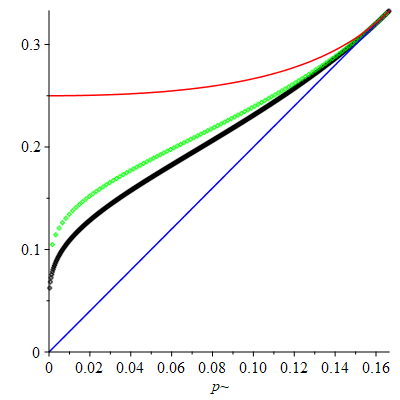
\includegraphics[width=8cm]{NumericPlot.png}
\caption{Numeric plot of the optimal proxy variance (black dots) for $0<p<\frac{1}{6}$. In blue is the variance $2p$ and in red is the upper bound $\sigma_{\text{up}}(p):=\frac{(1-2p)^2}{4(1-4p)}$. In green is the numeric evaluation of the upper bound $\sigma_{\text{up2}}^2$.}
\label{241029160152}
\end{figure}


\subsection{Refinements and comments}
It is easy to express $\sigma_{\text{opt}}^2$ in terms of $\lambda_c$. It gives a complicated equation for $\lambda_c$:
    \beq p\lambda_c \sinh \lambda_c -(1-2p+2p\cosh \lambda_c)\ln (1-2p+2p\cosh \lambda_c)=0\eeq 
    which to my knowledge does not admit explicit formulas but can easily be solved (and there is a unique zero on $(\lambda_0,+\infty)$) numerically. The knowledge of $\lambda_c$ implies then that
    \beq \sigma_{\text{opt}}^2=\frac{2p\sinh \lambda_c }{\lambda_c(2p \cosh \lambda_c +1-2p)} \eeq 

\medskip

The most important point is that we have two regimes which is quite unusual. For $p\in \big[\frac{1}{6},\frac{1}{2}\big)$ we have strict-Sub-Gaussianity while for $p\in \left(0,\frac{1}{6}\right)$ we no longer have sub-Gaussianity. This fact can be proved and also we can characterize the optimal proxy variance has the unique solution of a couple of equations. This can be solved numerically since we also have a lower bound (variance) and two upper bounds: one is simple but no so precise and the second one requires to solve numerically an explicit equation but is more precise. I think it gives a good story to tell. 

\medskip

Other cases that we may look after:
\begin{itemize}
    \item The case where we have $X(\Omega)=\{-a,0,a\}$ but with different probability in $-a$ and $a$ (i.e. $\P(X=-a)=p_1$ and $\P(X=a)=p_2$). In this case, we can also scale out $a$ so that we get two parameters. Be careful that the mean is no longer $0$ in this case. We get a compact space of parameters that is 2 dimensional so that we can at least give a plot of $\sigma_{\text{opt}}^2(p_1,p_2)$ as a $3D$ picture. Maybe the analysis can be carried out up to some extent. In particular the strict Sub-Gaussianity cases should be characterized.
    \item The generic case. After translation and dilation, we can take $X(\Omega)=\{-1,0,1+\epsilon\}$ with $\epsilon\in (-1,+\infty)$. In this case, we have $3$ parameters: $p_1$,$p_2$ and $\epsilon$. This complicates the numeric plots. The exact analysis seems also difficult but maybe we can find some conditions where to have strict-Sub-Gaussianity. 
\end{itemize}

\section{Olivier's proof extension}

Let $X$ be a random variable such that $X(\Omega)=\{-a,0,a\}$ and 
\begin{equation}
    \P(X=-a)=p_1\,,\, \P(X=0)=p_3 = 1-p_1-p_2\,,\, \P(X=a)=p_2
\end{equation}
where $p_1, p_2\in \left( 0,1\right) \text{ and since } p_3=0$ corresponds to two masses case  we will consider $p_3 > 0$ and $a>0$. We may define $Y=\frac{1}{a}X$ and use the fact that $\sigma_{\text{opt}}[X]=a \sigma_{\text{opt}}[X]$. Thus, we may restrict to $a=1$. We also may assume $p_2 \geq p_1$ and by considering $Y=-X$. We have
\beq \mu:=\E[Y]=-p_1+p_2 \geq 0\,\,,\,\, \sigma^2:=\text{Var}[Y]=p_1+p_2-(-p_1+p_2)^2\eeq
For any $\sigma>0$, we have that $\sigma$ is a variance proxy of $Y$ if and only if
\beq \E\left[e^{\lambda Y}\right]=p_1 e^{-\lambda }+ p_2e^{\lambda } +1-p_1-p_2\leq e^{(\frac{\lambda^2\sigma^2}{2}+\lambda \mu)} \,\, ,\,\, \forall \, \lambda\in \mathbb{R}\eeq
This inequality is equivalent to
\beq g_{\sigma,p}(\lambda):=\frac{\lambda^2\sigma^2}{2}-\ln(u_{0;p_1, p_2}(\lambda))+\lambda \mu \geq 0 \,\,,\,\,  \forall \, \lambda\in \mathbb{R}\eeq
With  $u_{0;p_1, p_2}(\lambda) := p_1e^{-\lambda}+p_2e^{\lambda}+1-p_1-p_2$ a smooth function and  $u_{0;p_1, p_2}(\lambda) > 0 \text{ , } \forall \lambda \in \mathbb{R}$. Thus the function $g_{\sigma,p}$ is a smooth function of $(\lambda,\sigma,p)$. For convenience we will use simply $u_0(\lambda)$ and we define
\beq u_{i}(\lambda)=u_{i-1}'(\lambda),   \  i  \in \{1,2,3\} \,\,,\,\,  \forall \, \lambda\in \mathbb{R}\eeq
We have $u_1(\lambda) = - p_1e^{-\lambda} + p_2e^{\lambda}$ and we observe that $u_2(\lambda) = u_0(\lambda)-p_3$, $u_3(\lambda) = u_1(\lambda)$ and $u_1^2(\lambda)=(u_0(\lambda)-p_3)^2-4p_1p_2$ for all $\lambda \in \mathbb{R}$ \\
%Since $g_{\sigma,p}$ is an even function of $\lambda$, this is equivalent to 
%\beq g_{\sigma,p}(\lambda):=\frac{\lambda^2\sigma^2}{2}-\ln( 2p\cosh \lambda +1-2p)\geq 0 \,\,,\,\,  %\forall \, \lambda\in \mathbb{R}_+\eeq
The general theory implies that $\text{Var}[Y]=p_1+p_2-(-p_1+p_2)^2$ is a lower bound for the optimal variance proxy. In other words, if $\sigma<\sqrt{p_1+p_2-(-p_1+p_2)^2}$ then $\sigma$ is not a variance proxy. Consequently, we shall only consider $\sigma \geq\sqrt{p_1+p_2-(-p_1+p_2)^2}$ in the following proof.
%\medskip

The function $g_{\sigma,p}$ a smooth function of $(\lambda,\sigma,p)$ and we have:

\bea g^{'}_{\sigma,p}(\lambda)&=&\lambda \sigma^2 -\frac{u_1(\lambda)}{u_0(\lambda)} + \mu \cr 
g^{(2)}_{\sigma,p}(\lambda)&=&\sigma^2-\frac{u_2}{u_0}+\frac{u_1^2}{u_0^2}= \sigma^2-\frac{u_2u_0-u_1^2}{u_0^2}\cr
&=&\sigma^2-\frac{u_0(u_0-p_3)-(u_0-p_3)^2   +4p_1p_2}{u_0^2}\cr
&=&\sigma^2-\frac{(u_0-p_3)(u_0-u_0+p_3)  +4p_1p_2}{u_0^2}  \cr
&=&\sigma^2-\frac{p_3u_0-p_3^2  +4p_1p_2}{u_0^2}  \cr
&=&\sigma^2-\frac{u_0(\lambda)p_3-p_3^2+4p_1p_2}{u_0(\lambda)^2}\cr
g^{(3)}_{p}(\lambda)&=&-\frac{u_1u_0 p_3}{u_0^3}+\frac{2(u_0p_3-p_3^2+4p_1p_2)}{u_0^3}\cr
&=&\frac{u_1}{u_0^3}\left(-u_0p_3+2u_0p_3-2p_3^2+8p_1p_2\right)\cr
&=&u_1(\lambda)\frac{p_3u_0(\lambda)+8p_1p_2-2p_3^2}{u_0(\lambda)^3}
\eea
Note in particular that $g^{(3)}_{p}$ does not depend on $\sigma$. Moreover, $g^{(3)}_{p}$ can be written as
\beq\label{g3} g^{(3)}_{p}(\lambda) = \frac{u_1(\lambda)N_{p_1,p_2}(\lambda)}{u_0(\lambda)^3} \eeq
where $N_{p_1,p_2}(\lambda) := p_3u_0(\lambda)+8p_1p_2-2p_3^2$. Observe that $u_0(\lambda)$ is strictly positive on $\mathbb{R}$. Therefore, the function $g^{(3)}$ and $N_{p_1, p_2} u_1$ share the same sign. We know that $u_1$ changes sign at $\lambda_0 := -\frac{1}{2}\ln(\frac{p_2}{p_1})$ assuming that $p_2\geq p_1$ we have $\lambda_0 \leq 0$. Hence, to determine the sign of $g^{(3)}$, it remains to analyze the sign of $N_{p_1, p_2}$. For this purpose, it is sufficient to  study the sign of the polynomial
\bea P(X) :=p_2p_3X^2+(8p_1p_2-p_3^2)X+p_3p_1, \text{where}\  X = e^{\lambda} > 0.\eea 
To determine the sign of $P(X)$, we compute its discriminant:
\bea \Delta = (p_3^2)^2 - 20p_1p_2(p_3)^2 + 64p_1^2p_2^2= (p_3^2-4p_1p_2)(p_3^2-16p_1p_2) \eea 
and it gives two different regimes that we shall study separately. In order to perform the study, we shall prove the following lemma.


\subsection{The case $p_3\leq 4\sqrt{p_1p_2}$}
In this case, we shall prove the following theorem.
\begin{theorem}[Explicit value of the optimal proxy variance for $p_3\leq 4\sqrt{p_1p_2}$]\label{TheoRegime1} When $p_3\leq 4\sqrt{p_1p_2}$, the optimal proxy variance is given by
\beq \sigma_{\text{opt}}^2= \frac{2(p_2-p_1)}{\ln \frac{p_2}{p_1}}\eeq
\end{theorem}

\begin{proof}Let us first observe that $\left(2\lambda_0,\sigma_{\text{opt}}^2\right)=\left(-\ln\frac{p_2}{p_1},\sigma_{\text{opt}}^2\right)$ is a solution $(\lambda,\sigma^2)$ of the system of equations
\beq g_{\sigma,p}(\lambda)=0 \text{ and } g^{'}_{\sigma,p}(\lambda) = 0\eeq
Moreover, the case $p_3\leq 4\sqrt{p_1p_2}$ is equivalent to the fact that $\Delta\leq 0$ or $\Delta>0$ with $P$ admitting two strictly negative roots (the sum of roots ($X_1,X_2)$ is $X_1+X_2 = \frac{p_3^2-8p_1p_2}{p_2p_3} < 0$ and the product of roots $X_1 X_2 = \frac{p_1}{p_2}>0$). Thus, the function $N_{p_1,p_2}$ is strictly positive on $\mathbb{R}$. Consequently, $g^{(3)}_{\sigma,p}$ and $u_1(\lambda)$ share the same sign and hence $g_{\sigma,p}^{(3)}$ is strictly negative on $(-\infty,\lambda_0)$ and strictly positive on $(\lambda_{0}, +\infty)$. Furthermore, since $\lim_{\lambda\to \pm \infty} g^{(2)}_{\sigma, p}(\lambda)=\sigma^2$, it follows that $\lambda_0$ is a global minimum of $g^{(2)}_{\sigma, p}$ with value $g^{(2)}_{\sigma,p}(\lambda_{0})=\sigma^2-\frac{2\sqrt{p_1p_2}}{p_3+2\sqrt{p_1p_2}}$. If $\sigma^2\geq\frac{2\sqrt{p_1p_2}}{p_3+2\sqrt{p_1p_2}}$ , then $g^{(2)}_{\sigma,p}$ is non-negative on $\mathbb{R}$ and so $g'_{\sigma,p}$ is a strictly increasing function. Since $g'_{\sigma,p}(0)=0$, $g'_{\sigma,p}$ is negative on $\mathbb{R}_-$ and positive on $\mathbb{R}_+$ and finally $g_{\sigma,p}$ has a global minimum at $\lambda=0$ which is precisely null so it is positive and $\sigma^2$ is a proxy variance. This gives that $\frac{2\sqrt{p_1p_2}}{p_3+2\sqrt{p_1p_2}}$ is an upper bound for the optimal proxy variance. 

On the contrary, if $\sigma^2<\frac{2\sqrt{p_1p_2}}{p_3+2\sqrt{p_1p_2}}$, then $g^{(2)}_{\sigma, p}$ has two distinct zeros $(\lambda_1(\sigma),\lambda_2(\sigma))$ such that $\lambda_1(\sigma)<\lambda_0<\lambda_2(\sigma)\leq 0$. Moreover, since $g_{\sigma,p}''(.;\sigma^2)$ is positive on $\mathbb{R}_+^*$, we get that $g_{\sigma,p}(.;\sigma^2)$ is always positive on $\mathbb{R}_+^*$ for any $\sigma^2\in \left(\text{Var}[Y],\frac{2\sqrt{p_1p_2}}{p_3+2\sqrt{p_1p_2}} \right) $. Since, we have observed that the equations $g_{\sigma,p}(\lambda,\sigma^2)=0=g_{\sigma,p}'(\lambda,\sigma^2)$ admits $\left(2\lambda_0,\frac{2(p_2-p_1)}{\ln \frac{p_2}{p_1}}\right)\in \mathbb{R}_-^*\times \left(\text{Var}[Y],+\infty\right)$ as solution, application of \autoref{LemmaNumber} on $\mathbb{R}_-^*$ implies that $g_{\sigma,p}(.;\sigma^2)$ is non-negative on $\mathbb{R}_-$ if and only if $\sigma^2\geq \frac{2(p_2-p_1)}{\ln \frac{p_2}{p_1}} $. Thus the optimal proxy variance in this case is $\sigma_{\text{opt}}^2= \frac{2(p_2-p_1)}{\ln \frac{p_2}{p_1}}$ . 

%\textcolor{blue}{Olivier: We could use \autoref{LemmaNumber} to simplify the discussion there. It is obvious that $g(.;\sigma^2)$ is non-negative on $\mathbb{R}_+^*$ (convex) and the lemma gives the result after observing the $(2\lambda_0;\frac{2(p_2-p_1)}{\ln \frac{p_2}{p_1}})$ is a solution. The lemma may also be used for the second regime in both $\mathbb{R}_-$ and $\mathbb{R}_+$ and \autoref{LemmaTechnicalGeneral} gives how to obtain the optimal proxy variance by comparing the two solutions. }

%On the contrary, if $\sigma^2<\frac{2\sqrt{p_1p_2}}{p_3+2\sqrt{p_1p_2}}$, then $g^{(2)}_{\sigma, p}$ has two distinct zeros $(\lambda_l,\lambda_r)$ such that $\lambda_l<\lambda_0<\lambda_r\leq 0$ because $g^{(2)}_{\sigma, p}(0)=\sigma^2-\text{Var}[Y]\geq 0$. This implies that $g'_{\sigma,p}$ is increasing on  $(-\infty, \lambda_l)$, then decreasing on $(\lambda_l, \lambda_r)$ and then increasing on $(\lambda_r, +\infty)$. Since $g'_{\sigma,p}(0)=0$ we must have $g'_{\sigma,p}(\lambda_r)<0$. Thus, since $\lim_{\lambda\to \pm \infty} g'_{\sigma,p}(\lambda)=\pm \infty$ and $g'_{\sigma,p}(0)=0$, we get only two cases:
%\begin{itemize}
%    \item If $g'_{\sigma,p}(\lambda_l)\leq 0$, then $g'_{\sigma,p}$ is negative on $\mathbb{R}_-$ and positive on $\mathbb{R}_+$ and since $g_{\sigma,p}(0)=0$, we end up with the fact that $g_{\sigma,p}$ is non-negative on $\mathbb{R}$.
%    \item If $g'_{\sigma,p}(\lambda_l)>0$, then $g'_{\sigma,p}$ has three distinct zeros: $(\lambda_-,\lambda_+,0)$ such that $\lambda_-<\lambda_l<\lambda_+<\lambda_r$. Thus $g_{\sigma,p}$ is decreasing on $(-\infty, \lambda_-)$, then increasing on $(\lambda_-,\lambda_+)$, decreasing on $(\lambda_+,0)$ and then increasing on $(0,+\infty)$. Since $g_{\sigma,p}(0)$, $g_{\sigma,p}$ is obviously positive on $\mathbb{R}_+$ and $g_{\sigma,p}(\lambda_+)>0$. Consequently, $g_{\sigma,p}$ is non-negative on $\mathbb{R}$ if and only if $g_{\sigma,p}(\lambda_-)\geq 0$. 
%\end{itemize}
%Let us now conclude this case by observing that $\frac{d}{d\sigma}[g'_{\sigma,p}(\lambda_l)]= g''_{\sigma,p}(\lambda_l) \frac{d}{d\sigma}[\lambda_l] + 2\lambda_l\sigma=2\lambda_l\sigma<0$. Thus, when lowering $\sigma^2$ from $\frac{2\sqrt{p_1p_2}}{p_3+2\sqrt{p_1p_2}}$ down to $\text{Var}[Y]$, we necessarily face the second situation mentioned above. Finally, in this situation we also have $\frac{d}{d\sigma}[g_{\sigma,p}(\lambda_-)]= g'_{\sigma,p}(\lambda_-)\frac{d}{d\sigma}[\lambda_-]+ \lambda_-^2\sigma=\lambda_-^2\sigma>0$ so that $g_{\sigma,p}(\lambda_-)$ is a strictly decreasing function of $\sigma$. This allows to conclude that the optimal proxy variance is characterized as the unique solution $(\lambda_c,\sigma_{\text{opt}}^2)$ of the system
%\small{\beq g_{\sigma_{\text{opt}},p}(\lambda_c)=0\,,\, g^{'}_{\sigma_{\text{opt}},p}(\lambda_c)=0\,\,,\,\, \lambda_c<\lambda_0=-\frac{1}{2}\ln\frac{p_2}{p_1}\,\,,\,\, \sigma_{\text{opt}}^2\in \left[\text{Var}[Y], \frac{2\sqrt{p_1p_2}}{p_3+2\sqrt{p_1p_2}}\right]\eeq}
%\normalsize{Eventually}, the observation made above that $\left(2\lambda_0,\frac{2(p_2-p_1)}{\ln \frac{p_2}{p_1}}\right)$ is a solution of the previous system gives by uniqueness that $\lambda_c=2\lambda_0$ and $\sigma_{\text{opt}}^2=\frac{2(p_2-p_1)}{\ln \frac{p_2}{p_1}}$ ending the proof.
\end{proof}

\autoref{TheoRegime1} implies the following corollary.

\begin{corollary}\label{StrictSub-GaussianityRegime1} For $p_3\leq 4\sqrt{p_1p_2}$, the random variable $Y$ is strictly Sub-Gaussian if and only if $p_1=p_2=p$. In this symmetric case, the condition $p_3\leq 4\sqrt{p_1p_2}$ is equivalent to $p\geq \frac{1}{6}$. 
\end{corollary}

\begin{proof}The proof is obvious from the fact that in this case $\sigma_{\text{opt}}^2=\frac{2(p_2-p_1)}{\ln \frac{p_2}{p_1}}\geq \text{Var}[Y]=p_1+p_2-(p_2-p_1)^2$ with equality if and only if $p_1=p_2$.
\end{proof}

\begin{figure}[H]
\centering
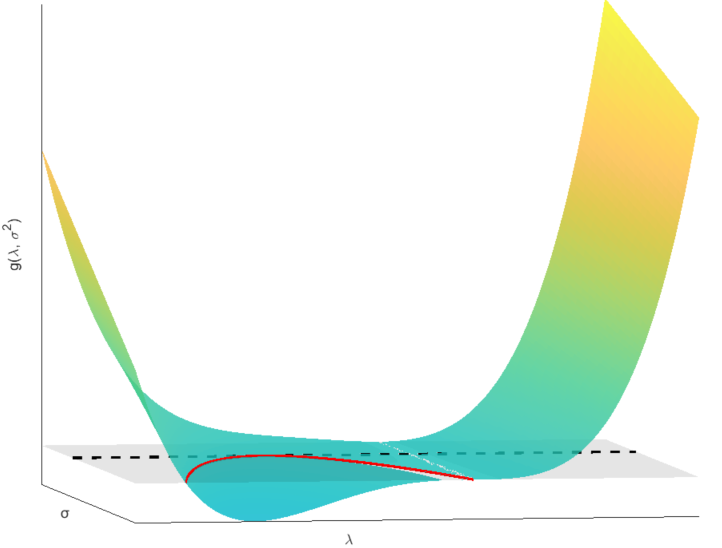
\includegraphics[width=8cm]{g_plot_p1p2-1325.png}
\caption{Numeric plots of $g_{\sigma,p}$ function for fixed $p=(0.13, 0.25)$ varying $\lambda$  and $\sigma^2$ from variance to upper bound $\sigma_{up}$}
\label{241029160153}
\end{figure}

\textcolor{red}{We should add some plots of the function $g_{\sigma,p}$ for some given values of $(p_1,p_2)$ with varying $\sigma^2$ from the upper bound down to the variance. It is first convex, then now longer convex but with no oscillation and then starts oscillating until it reaches the optimal value. When we hit the variance, it becomes obviously negative locally around $0_-$.}

%\textcolor{red}{Note that $\Delta$ is itself a quadratic polynomial in  $p_3^2$. Denoting its discriminant by $\Delta_{p_3}$to fully characterize its sign.
%\bea \Delta_{p_3} = (-20p_1p_2)^2-256p_1^2p_2^2 = (12p_1p_2)^2 > 0 \eea
%Since $\Delta_{p_3}>0$, the equation $\Delta = 0$ has two distinct real roots, $p_3^2 = 4p_1p_2$  and   $p_3^2 = 16p_1p_2$, thus $\Delta$ can be written as:
%\bea \Delta = (p_3^2-4p_1p_2)(p_3^2-16p_1p_2).\eea}
%Because  the leading coefficient of $\Delta$ is positive, it follows that $\Delta > 0$ when $p_3>4\sqrt{p_1p_2} \text{ or }p_3<2\sqrt{p_1p_2}$ and $\Delta < 0$ otherwise. In the case $\Delta < 0$, the polynomial $P(X)$ is strictly positive for all X, thus $N_{p_1, p_2}(\lambda)$ is strictly positive for all $\lambda \in \mathbb{R}.$\\

\subsection{The case $p_3>4\sqrt{p_1p_2}$}
In this case, we have $\Delta>0$ and $P$ has two distinct positive roots $0<X_-<X_+$ so that $N_{p_1,p_2}$ has exactly two roots $\lambda_-<\lambda_+$. Their location is given by the following lemma.

\newtheorem*{manuallemma}{Lemma 1.1}
\begin{manuallemma}
\label{lemma:lambda_ordering}
Let $p_1, p_2 \in \mathbb{R}$ such that $p_2 \geq p_1$ and $p_3^2>16p_1p_2$. Then the following inequality holds:
\[
\lambda_0 \leq 0 <\lambda_- <   \lambda_+
\]
\end{manuallemma}
\begin{proof}Let us first observe that we have:
\bea \lambda_{-}= \ln\left(\frac{p_3^2-8p_1p_2 - \sqrt{(p_3^2-4p_1p_2)(p_3^2-16p_1p_2)}}{2p_1p_2}\right) \cr \lambda_{+} =\ln\left(\frac{p_3^2-8p_1p_2 +  \sqrt{(p_3^2-4p_1p_2)(p_3^2-16p_1p_2)}}{2p_1p_2}\right) \eea
%we have $\sqrt{(p_3^2-4p_1p_2)(p_3^2-16p_1p_2)} > 0$ and $p_3^2-8p_1p_2 > 8p_1p_2$ thus  $p_3^2-8p_1p_2 +  \sqrt{(p_3^2-4p_1p_2)(p_3^2-16p_1p_2)} > 8p_1p_2$ thus $\lambda_+>\ln(4)$ and as $\lambda_0 \leq 0$ we conclude $\lambda_+>\lambda_0$\\
We shall denote for compactness $x := p_3^2>0$, $y := p_1p_2>0$ so that we have the condition $x>16y$. Since $\lambda_0<0$, we only need to prove that $\lambda_->0$. We will now prove that $\lambda_{-} > 0$ under the condition $x > 16y>0$. To establish this result, we proceed through a chain of equivalent inequalities, beginning with the definition of $\lambda_{-}$
\begin{align*}
\lambda_{-} > 0 
&\iff \frac{x - 8y - \sqrt{(x-4y)(x-16y)}}{2y} > 1 \\
&\iff x - 8y - \sqrt{(x-4y)(x-16y)} > 2y \\
&\iff x - 10y > \sqrt{(x-4y)(x-16y)} \\
&\iff (x - 10y)^2 > (x-4y)(x-16y) \quad (\text{because } x > 16y \Rightarrow x-10y > 6y > 0) \\
&\iff x^2 - 20xy + 100y^2 > x^2 - 20xy + 64y^2 \\
&\iff 100y^2 > 64y^2 \\
&\iff 36y^2 > 0 \quad (\text{always valid for  } y \neq 0)
\end{align*}
Thus we get  $\lambda_0 < 0 <\lambda_- <   \lambda_+$ under the condition $p_3^2>16p_1p_2$ ending the proof of the lemma.  
\end{proof}
%\begin{proof}The proof is done by straightforward computations and inequalities and is presented in \autoref{AppendixLemma}.
%\end{proof}

We shall now use split the analysis of the sign of $g(.;\sigma^2)$ on $\mathbb{R}_-^*$ and $\mathbb{R}_+^*$. Let us first observe that the discussion made for $\mathbb{R}_-^*$ in the proof of \autoref{TheoRegime1} is still valid. Thus, $g(.;\sigma^2)$ is non-negative on $\mathbb{R}_-^*$ if and only if $\sigma^2\geq \frac{2(p_2-p_1)}{\ln \frac{p_2}{p_1}}$. Let us now discuss the situation on $\mathbb{R}_+^*$. From \autoref{lemma:lambda_ordering} and \eqref{g3} we get that $g^{(3)}$ is negative on $(-\infty,\lambda_0)\cup\left(\lambda_-(\sigma),\lambda_+(\sigma)\right)$  and positive on $(\lambda_0,\lambda_-(\sigma))\cup\left(\lambda_+(\sigma),+\infty\right)$. Consequently, $g''(.;\sigma^2)$ is increasing on $(0,\lambda_-)$ and since $g''(0;\sigma^2)=0$ is it thus positive on this interval. Then, $g''(.;\sigma^2)$ is decreasing on $(\lambda_-(\sigma),\lambda_+(\sigma))$ and then increasing on $(\lambda_+(\sigma),+\infty)$ with $g''(+\infty;\sigma^2)=\sigma^2>0$. Thus, there are only two possible cases: either $g''(\lambda_+(\sigma);\sigma^2)\geq 0$ and then $g(.;\sigma^2)$ is strictly convex and positive on $\mathbb{R}_+^*$ or $g''(\lambda_+(\sigma);\sigma^2)<0$ in which case $g''(.\sigma^2)$ has exactly two zeros $(\lambda_1(\sigma),\lambda_2(\sigma))$ on $\mathbb{R}_+^*$ such that $\lambda_-(\sigma)<\lambda_1(\sigma)<\lambda_+(\sigma)<\lambda_2(\sigma)$. We may thus apply \autoref{LemmaNumber} whose conclusion depends on the existence of a solution $(\lambda,\sigma^2)\in \left(\lambda_-,+\infty\right)*\times \left(\text{Var}[Y],+\infty\right)$ of the equation $g(\lambda;\sigma^2)=0=g'(\lambda;\sigma^2)$. This set of equations is equivalent to
\beq \sigma^2=\frac{1}{\lambda}\left(\frac{u_1(\lambda)}{u_0(\lambda)}-\mu\right)=\frac{1}{\lambda}\left(p_1-p_2+\frac{p_2e^\lambda-p_1e^{-\lambda}}{p_1e^{-\lambda}+p_2e^{\lambda}+1-p_1-p_2}\right)
\eeq
and $\lambda$ positive solution of
\beq \lambda \frac{u_1(\lambda)}{u_0(\lambda)}- 2\ln (u_0(\lambda))+\lambda \mu=0\eeq
i.e.
\beq \label{EqF} F(\lambda):=\lambda u_1(\lambda)-2u_0(\lambda)\ln u_0(\lambda)+ \lambda u_0(\lambda)(p_2-p_1)=0\eeq
From \autoref{LemmaNumber2}, $F(\lambda)=0$ has no solution on $\mathbb{R}_+^*$ such that $\sigma^2=\frac{1}{\lambda}\left(\frac{u_1(\lambda)}{u_0(\lambda)}-\mu\right)<\text{Var}[Y]$. Thus, we have two cases:
\begin{itemize}
    \item If $F$ has a positive zero $\lambda_c>0$ then \autoref{LemmaNumber} implies that this zero is unique on $\mathbb{R}_+^*$ and we get that $\sigma_c^2=\frac{1}{\lambda_c}\left(\frac{u_1(\lambda_c)}{u_0(\lambda_c)}-\mu\right)\geq\text{Var}[Y]$. \autoref{GeneralCharac} implies that the optimal proxy variance is given by
    \beq \sigma_{\text{opt}}^2=\text{Max}\left(\frac{2(p_2-p_1)}{\ln \frac{p_2}{p_1}}, \frac{1}{\lambda_c}\left(\frac{u_1(\lambda_c)}{u_0(\lambda_c)}-(p_2-p_1)\right) \right)\eeq
    \item If $F$ has no zero on $\mathbb{R}_+^*$ then $g(.;\sigma^2)$ is positive on $\mathbb{R}_+^*$ and thus the optimal proxy variance is given by $\sigma^2_{\text{opt}}=\frac{2(p_2-p_1)}{\ln \frac{p_2}{p_1}}$.
\end{itemize}

\begin{remark}Note that $\underset{\lambda\to +\infty}{\lim} F(\lambda)=-\infty$ and $F(\lambda)=\frac{1}{6}M_3[Y]\lambda^3+\frac{1}{4}\left(\frac{1}{3}M_4[Y]-\text{Var}[Y]^2\right)\lambda^4+ O(\lambda^5)$, where $M_3:=\mathbb{E}[(Y-\mu)^3]$ and $M_4:=\mathbb{E}[(Y-\mu)^4]$. Thus, a sufficient condition for $F$ to admit a positive zero is that $M_3[Y]>0$ or $\left[M_3[Y]=0 \text{ and } \frac{1}{3}M_4[Y]\text{Var}[Y]^2>0\right]$. In particular for $p_1=p_2=p$, we have that $F(\lambda)=\frac{1}{6}p(1-6p)\lambda^4+O(\lambda^5)$ so that for $p>\frac{1}{6}$ (which is the equivalent condition to $p_3>4\sqrt{p_1p_2}$ in this case) $F$ always has a unique positive zero $\lambda_c$ and the corresponding variance $\sigma_c^2=\frac{1}{\lambda_c}\frac{u_1(\lambda_c)}{u_0(\lambda_c)}$ is always greater than $2p=\text{Var}[Y]$ and hence the optimal proxy variance is always $\sigma_{\text{opt}}^2=\sigma_c^2=\frac{1}{\lambda_c}\frac{u_1(\lambda_c)}{u_0(\lambda_c)}$ in the symmetric case $p_1=p_2=p$.
\end{remark}


\textcolor{red}{Olivier: There are cases where $F$ does not admit a positive zero. For example $(p_1,p_2)=(0.01, 0.5)$ which belongs to the second regime. }

\medskip

\textcolor{red}{To be done: General theorem tells us that the optimal proxy variance selects the biggest value of $\sigma^2$. However, apart from the symmetric case which is dealt with in the previous remark, it is not even clear that there is a positive zero of $F$ in the second regime. I have plots where the zero exists and some where it does not. Logically, there should also be cases for which the zero exists but the corresponding variance is not the biggest one. Therefore, at this stage it would be good to have a 3d plot of the optimal variance relatively to $(p_1,p_2)$. When $p_1+p_2=1/3$, we have $\sigma_c^2=\frac{2(p_2-p_1)}{\ln \frac{p_2}{p_1}}$ and the positive zero is $\lambda_c=\ln(p_2/p_1)>0$. This is a case where both critical variance are equal so this also possible even in the non-symmetric case.}

\newpage
\section{Dirac comb}
\subsection{Naive case}
Let \( X \sim \mathcal{U}(\{1, 2, \dots, N\}) \) be a discrete random variable uniformly distributed over the set $ \mathcal{I} = \{1, 2, \dots, N\}$. Its probability mass function is given by
\[
\mathbb{P}(X = k) = \frac{1}{N}, \quad \text{for all } k \in \{1, 2, \dots, N\}.
\]
The distribution of \( X \) can be written as a uniform mixture of Dirac measures:
\[
\mathbb{P}_X = \frac{1}{N} \sum_{k=1}^N \delta_k, \text{ ,  where   } \delta_{k} \text{  denotes the Dirac mass centered at } k
\]

and we have  \beq \mu:=\E[X]=\frac{N+1}{2}\,\,,\,\, \sigma^2:=\text{Var}[X]=\frac{N^2-1}{12}, \ \ \ \kappa_3=\text{Skew}[X]=0 \eeq
For any $\sigma>0$, we have that $\sigma$ is a variance proxy of $X$ if and only if \beq \label{eq:mgf_inequality} \E\left[e^{\lambda X}\right]=  \frac{1}{N}\sum_{k=1}^{N} e^{\lambda k} \leq e^{(\frac{\lambda^2\sigma^2}{2}+\lambda \mu)} \,\, ,\,\, \forall \, \lambda\in \mathbb{R}\eeq This inequality is equivalent to \beq g_{\sigma,p}(\lambda):=\frac{\lambda^2\sigma^2}{2}-u(\lambda)+\lambda \frac{N+1}{2} \geq 0 \,\,,\,\,  \forall \, \lambda\in \mathbb{R}\eeq With  $u(\lambda) := \ln\left(\frac{1}{N}\sum_{k=1}^{N} e^{\lambda k}\right)$ being a smooth function and we have.\\
\bea g^{'}_{\sigma,p}(\lambda) &=& \lambda \sigma^2 -u^{'}(\lambda) + \mu \,\,,\,\ \cr 
g^{(2)}_{\sigma,p}(\lambda) &=& \sigma^2 -u^{(2)}(\lambda),  \forall \, \lambda\in \mathbb{R}. \eea The general theory implies that $\text{Var}[X]=\frac{N^2-1}{12}$ is a lower bound for the optimal variance proxy. In other words, if $\sigma<\sqrt{\frac{N^2-1}{12}}$ then $\sigma$ is not a variance proxy. Consequently, we shall only consider $\sigma\geq \sqrt{\frac{N^2-1}{12}}$ in the following proof.\\Let us define the discrete probability distribution  $P_{\lambda}$ on $\mathcal{I}$ , such that: \beq P_{\lambda}(k) = \frac{e^{\lambda k}}{\sum_{j=1}^{N} e^{\lambda j}} \ \ \ \text{ and } \mathbb{E_{\lambda}}[k] = {\sum_{j=1}^{N}j P_{\lambda}[j]}\eeq 
Note that for $\lambda=0 , \ \ P_\lambda$ is equivalent to $X$.\\
\begin{lemma}[Symmetry of Tilted Probabilities]\label{lem:symmetry}
For any $\lambda \in \mathbb{R}$ and $k \in \{1,\ldots,N\}$:
\begin{equation}
P_{-\lambda}(k) = P_{\lambda}(N-k+1)
\end{equation}
\end{lemma}

\begin{proof}
We compute directly:
\begin{align*}
P_{-\lambda}(k) &= \frac{e^{-\lambda k}}{\sum_{j=1}^N e^{-\lambda j}} \\
&= \frac{e^{\lambda (N - k + 1)} \cdot e^{-\lambda (N + 1)}}{\sum_{j=1}^N e^{\lambda (N - j + 1)} \cdot e^{-\lambda (N + 1)}}  \\
&= \frac{e^{\lambda (N - k + 1)}}{\sum_{m=1}^N e^{\lambda m}} \quad \text{(setting $m = N-j+1$)} \\
&= P_{\lambda}(N - k + 1). 
\end{align*}
\end{proof}

\begin{lemma}[Expectation Symmetry]\label{lem:expectation}
The expected values satisfy:
\begin{equation}
\mathbb{E}_{-\lambda}[X] = N + 1 - \mathbb{E}_{\lambda}[X]
\end{equation}
\end{lemma}

\begin{proof}
Using Lemma \ref{lem:symmetry} and a change of variables:
\begin{align*}
\mathbb{E}_{-\lambda}[X] &= \sum_{k=1}^N k P_{-\lambda}(k) \\
&= \sum_{k=1}^N k P_{\lambda}(N - k + 1) \\
&= \sum_{m=1}^N (N - m + 1) P_{\lambda}(m) \quad \text{(with $m = N - k + 1$)} \\
&= (N + 1)\sum_{m=1}^N P_{\lambda}(m) - \sum_{m=1}^N m P_{\lambda}(m) \\
&= (N + 1) - \mathbb{E}_{\lambda}[X]. 
\end{align*}
\end{proof}

\begin{proposition}[Variance Parity]\label{prop:variance}
The variance is an even function of $\lambda$:
\begin{equation}
\text{Var}_{-\lambda}[X] = \text{Var}_{\lambda}[X]
\end{equation}
\end{proposition}

\begin{proof}
We compute the variance under $-\lambda$:
\begin{align*}
\text{Var}_{-\lambda}[X] &= \mathbb{E}_{-\lambda}[X^2] - (\mathbb{E}_{-\lambda}[X])^2 \\
&= \left[\sum_{k=1}^N k^2 P_{-\lambda}(k)\right] - \left[N + 1 - \mathbb{E}_{\lambda}[X]\right]^2 \\
&= \left[\sum_{m=1}^N (N - m + 1)^2 P_{\lambda}(m)\right] - \left[(N + 1)^2 - 2(N + 1)\mathbb{E}_{\lambda}[X] + (\mathbb{E}_{\lambda}[X])^2\right] \\
&= \left[(N + 1)^2 \sum_{m=1}^N P_{\lambda}(m) - 2(N + 1)\sum_{m=1}^N k P_{\lambda}(m) + \sum_{m=1}^N k^2 P_{\lambda}(m)\right] 
- \left[(N + 1)^2 - 2(N + 1)\mathbb{E}_{\lambda}[X] + (\mathbb{E}_{\lambda}[X])^2\right] \\
&= \left[(N + 1)^2 - 2(N + 1)\mathbb{E}_{\lambda}[X] + \mathbb{E}_{\lambda}[X^2]\right]
- \left[(N + 1)^2 - 2(N + 1)\mathbb{E}_{\lambda}[X] + (\mathbb{E}_{\lambda}[X])^2\right] \\
&= \mathbb{E}_{\lambda}[X^2] - (\mathbb{E}_{\lambda}[X])^2 \\
&= \text{Var}_{\lambda}[X].
\end{align*}
where we used Lemma \ref{lem:expectation} for the expectation terms.
\end{proof}

\begin{lemma}[Derivatives of Log-Partition Function as Moments]\label{lem:log_partition_moments}
Let 
\[
u(\lambda) = \ln\left(\sum_{j=1}^{N} e^{\lambda j}\right)
\]
Then the derivatives of \( u(\lambda) \) give the moments of the associated exponential family distribution:
\begin{align}
u'(\lambda) &= \mathbb{E}_{\lambda}[X] \\
u''(\lambda) &= \text{Var}_{\lambda}[X] \\
u^{(3)}(\lambda) &=  \text{Skew}_{\lambda}[X]
\end{align}
\end{lemma}

\begin{proof}
We compute the derivative of the expectation:
\begin{align*}
\label{eq:var}
u^{'}(\lambda) &= \frac{\frac{d}{d\lambda}(\sum_{j=1}^{N} e^{\lambda j})}{\sum_{j=1}^{N} e^{\lambda j}}\\
&= \sum_{j=1}^{N} j \frac{e^{\lambda j}}{\sum_{j=1}^{N} e^{\lambda j}} \\
& = \mathbb{E}_{\lambda}[X] \\
u^{(2)}(\lambda) &= \frac{d}{d\lambda}\left(\frac{\sum_{j=1}^{N} j e^{\lambda j}}{\sum_{j=1}^{N} e^{\lambda j}}\right) \\ 
&= \frac{\sum_{j=1}^{N} j^2 e^{\lambda j} \sum_{j=1}^{N} e^{\lambda j} - \left(\sum_{j=1}^{N} j e^{\lambda j}\right)^2} {\left(\sum_{j=1}^{N} e^{\lambda j}\right)^2} \\
&= \sum_{j=1}^{N} j^2 \frac{e^{\lambda j}}{\sum_{i=1}^{N} e^{\lambda i}} - \left(\sum_{j=1}^{N} j\frac{e^{\lambda j}}{\sum_{i=1}^{N} e^{\lambda i}}\right)^2 \\ 
&= \sum_{j=1}^{N} j^2 P_{\lambda}[j] - \left(\sum_{j=1}^{N} j P_{\lambda}[j]\right)^2 \\
&= \mathbb{E}_{\lambda}[X^2] - \left(\mathbb{E}_{\lambda}[X]\right)^2 \\
&= \text{Var}_{\lambda}[X] \\ 
u^{(3)}(\lambda) &= \frac{d}{d\lambda} \text{Var}_{\lambda}[X] \\
&= \frac{d}{d\lambda} \left(\mathbb{E}_{\lambda}[X^2] - (\mathbb{E}_{\lambda}[X])^2\right) \\
&= \left(\mathbb{E}_{\lambda}[X^3] - \mathbb{E}_{\lambda}[X]\mathbb{E}_{\lambda}[X^2]\right) - 2\mathbb{E}_{\lambda}[X]\left(\mathbb{E}_{\lambda}[X^2] - (\mathbb{E}_{\lambda}[X])^2\right) \\
&= \mathbb{E}_{\lambda}[X^3] - 3\mathbb{E}_{\lambda}[X]\mathbb{E}_{\lambda}[X^2] + 2(\mathbb{E}_{\lambda}[X])^3 \\
&= \mathbb{E}_{\lambda}[(X - \mathbb{E}_{\lambda}[X])^3]\\
&=\text{Skew}_{\lambda}[X]
\end{align*}
\end{proof}


From  Lemma~\ref{lem:log_partition_moments} it follows that the skewness is given by: \beq \text{Skew}_{\lambda}[X] = \frac{d}{d\lambda}\text{Var}_{\lambda}[X]\eeq Since $\text{Var}_{\lambda}[X]$ is an even function of $\lambda$, its derivative $\text{Skew}_{\lambda}[X]$ is odd. Consequently, the analysis of $\text{Skew}_{\lambda}[X]$ can be restricted to $\mathbb{R}_+$.\\
\begin{lemma}[Explicit Moments via the Log-Partition Function]\label{lem:explicit_moments}
Let \( X \in \{1, 2, \dots, N\} \) for some integer \( N \geq 2 \), and let the exponential family distribution be defined by:
\[
P_{\lambda}(k) = \frac{e^{\lambda k}}{Z(\lambda)}, \quad \text{where} \quad Z(\lambda) = \sum_{k=1}^N e^{\lambda k} \quad \text{and} \quad u(\lambda) = \ln(Z(\lambda)).
\]
Then, the log-partition function and its first three derivatives are given by:
\begin{align*}
u(\lambda) &= \lambda + \ln(1 - e^{\lambda N}) - \ln(1 - e^{\lambda}), \\
u'(\lambda) &= 1 - \frac{N e^{\lambda N}}{1 - e^{\lambda N}} + \frac{e^{\lambda}}{1 - e^{\lambda}} = \mathbb{E}_{\lambda}[X], \\
u''(\lambda) &= -\frac{N^2 e^{\lambda N}}{(1 - e^{\lambda N})^2} + \frac{e^{\lambda}}{(1 - e^{\lambda})^2} = \text{Var}_{\lambda}[X], \\
u^{(3)}(\lambda) &= -\frac{N^3 e^{\lambda N}(1 + e^{\lambda N})}{(1 - e^{\lambda N})^3} + \frac{e^{\lambda}(1 + e^{\lambda})}{(1 - e^{\lambda})^3} = \mathbb{E}_{\lambda}[(X - \mathbb{E}_{\lambda}[X])^3].
\end{align*}
\end{lemma}

\begin{proof}
The partition function is a finite geometric series:
\[
Z(\lambda) = \sum_{k=1}^N e^{\lambda k} = e^{\lambda} \cdot \frac{1 - e^{\lambda N}}{1 - e^{\lambda}}.
\]
Taking the logarithm:
\[
u(\lambda) = \ln Z(\lambda) = \lambda + \ln(1 - e^{\lambda N}) - \ln(1 - e^{\lambda}).
\]

\textbf{First derivative:}
\begin{align*}
u'(\lambda) &= 1 + \frac{d}{d\lambda} \ln(1 - e^{\lambda N}) - \frac{d}{d\lambda} \ln(1 - e^{\lambda}) \\
&= 1 - \frac{N e^{\lambda N}}{1 - e^{\lambda N}} + \frac{e^{\lambda}}{1 - e^{\lambda}}
\end{align*}

\textbf{Second derivative:}
\begin{align*}
u''(\lambda)
&= -\frac{N^2 e^{\lambda N}}{(1 - e^{\lambda N})^2} + \frac{e^{\lambda}}{(1 - e^{\lambda})^2}
\end{align*}

\textbf{Third derivative:}
Differentiating again:
\begin{align*}
u^{(3)}(\lambda)
&= -\frac{d}{d\lambda} \left( \frac{N^2 e^{\lambda N}}{(1 - e^{\lambda N})^2} \right)
+ \frac{d}{d\lambda} \left( \frac{e^{\lambda}}{(1 - e^{\lambda})^2} \right) \\
&= -\frac{N^3 e^{\lambda N}(1 + e^{\lambda N})}{(1 - e^{\lambda N})^3} + \frac{e^{\lambda}(1 + e^{\lambda})}{(1 - e^{\lambda})^3}
\end{align*}

\end{proof}

\begin{proposition}[Negativity of the Third Derivative of the Log-Partition Function]\label{prop:neg_third_deriv}
Let \( N \geq 2 \) be an integer and let \( \lambda > 0 \) be a real number. Then the third derivative of the log-partition function is strictly negative. In other words,
\[
u^{(3)}(\lambda) = -\frac{N^3 e^{\lambda N}(1 + e^{\lambda N})}{(1 - e^{\lambda N})^3} + \frac{e^{\lambda}(1 + e^{\lambda})}{(1 - e^{\lambda})^3} < 0.
\]
Consequently,
\[
\text{Skew}_{\lambda}[X] < 0 \text{ for all } \lambda \in \mathbb{R}_+^*
\]
\end{proposition}
\begin{proof}
Let us consider the auxiliary function
\[
f(t) = \frac{t(t + 1)}{(1 - t)^3}, \quad \text{where} \quad t = e^{\lambda} > 1.
\]

We compute the derivative:
\[
f'(t) = \frac{1 + 4t + t^2}{(1 - t)^4}.
\]

Since both the numerator and denominator are strictly positive for all \( t > 1 \), it follows that \( f'(t) > 0 \). Therefore, \( f \) is strictly increasing on the interval \( (1, +\infty) \).

Now fix \( \lambda > 0 \), so that \( t = e^{\lambda} > 1 \). Since \( N \geq 2 \), we have \( t^N > t \), and by monotonicity of \( f \),
\[
f(t^N) > f(t),
\]
i.e.,
\[
\frac{e^{\lambda N}(1 + e^{\lambda N})}{(1 - e^{\lambda N})^3} > \frac{e^{\lambda}(1 + e^{\lambda})}{(1 - e^{\lambda})^3}.
\]

As \( N^3 \geq 8 \) (since \( N \geq 2 \)), we get:
\[
\frac{N^3 e^{\lambda N}(1 + e^{\lambda N})}{(1 - e^{\lambda N})^3} > \frac{e^{\lambda}(1 + e^{\lambda})}{(1 - e^{\lambda})^3}.
\]

Therefore,
\[
u^{(3)}(\lambda) 
= - \frac{N^3 e^{\lambda N}(1 + e^{\lambda N})}{(1 - e^{\lambda N})^3}
+ \frac{e^{\lambda}(1 + e^{\lambda})}{(1 - e^{\lambda})^3}
< 0,
\]
which completes the proof.
\end{proof}


%\begin{proposition}\label{prop:expectation}
%Let \( N \geq 2 \) be an integer and let \( \lambda > 0 \) be a real number. Then the following inequality holds:
%\[
%\mathbb{E}_{\lambda}[X]  > \frac{N+1}{2}.
%\]
%\end{proposition}

%\begin{proof}
%From Lemma~\ref{lem:log_partition_moments} we have: $u''(\lambda) = \text{Var}_{\lambda}[X] > 0$ for all $\lambda \in \mathbb{R}$  and in particular for \( \lambda \geq 0 \). This implies that \( u'(\lambda) = \mathbb{E}_{\lambda}[X] \) is strictly increasing in \( \lambda \).
%At \( \lambda = 0 \). The distribution  \( \mathbb{P}_0[X] \) becomes uniform over \( \{1, \dots, N\} \), and $\mathbb{E}_0[X] = \frac{N+1}{2}$ .Since \( \mathbb{E}_{\lambda}[X] \) is strictly increasing in \( \lambda \) and \( \lambda > 0 \), it follows that:
%\[
%\mathbb{E}_{\lambda}[X] > \mathbb{E}_{0}[X] = \frac{N+1}{2}.
%\]
%\end{proof} 
\subsection{Variance Proxy Optimality}
From Proposition~\ref{prop:variance}, we know that $\text{Var}_{\lambda}[X]$ is an even function of $\lambda$. This symmetry allows us to restrict the analysis in $\mathbb{R}_+$. Furthermore, Proposition~\ref{prop:neg_third_deriv} states that: \beq \text{Skew}_{\lambda}[X] < 0 , \ \ \forall \lambda > 0\eeq Given the derivative relationship $\text{Skew}{\lambda}[X] = \frac{d}{d\lambda}\text{Var}{\lambda}[X]$, along with the evenness of the variance, it follows that the skewness is an odd function: \beq \text{Skew}_{\lambda}[X] = \frac{d}{d\lambda}\text{Var}_{\lambda}[X] \eeq
Consequently $\text{Var}_{\lambda}[X]$ is increasing on $\mathbb{R}_-$, and decreasing on $\mathbb{R_+}$, and attains a unique global maximum at $\lambda=0$.\\
Now consider the function \bea g^{(2)}(\lambda) &=& \sigma^2 - u^{(2)}(\lambda) \cr
&=& \sigma^2 - \text{Var}_{\lambda}[X] \cr
&\geq& \sigma^2 - \text{Var}_0[X] \cr
&\geq&  \sigma^2 - \text{Var}[X] \cr
&\geq& 0 \eea
Where equality holds if and only if $\lambda=0$.\\
The system of equations \beq g_{\sigma,p}(\lambda,\sigma^2)=0=g_{\sigma,p}'(\lambda,\sigma^2) \eeq admits a unique solution at $\lambda = 0$.  Moreover, $g$ attains a global unique minimum at $\lambda = 0$, confirming that $\sigma^2$ is a valid variance proxy. This argument is valid for any $\sigma^2\geq \text{Var}[X]=\frac{N^2-1}{12}$. Therefore, the optimal proxy variance is: \beq \sigma^2_{opt}[X]=\text{Var}[X]=\frac{N^2-1}{12}\eeq 
which implies that \textbf{$X$ is strictly Sub-Gaussian}

\subsection{Dirac comb Generalization}
Let consider X a discrete random variable taking real values in finite equidistant set \( \mathcal{S} = \{x_1, x_2, \ldots, x_N\} \subset \mathbb{R} \), where \( x_i = a + (i-1)h \) for some fixed \( a \in \mathbb{R} \) and spacing \( h > 0 \). Suppose \( X \) has associated probability vector \( p = (p_1, p_2, \ldots, p_K) \), where \( p_i = \mathbb{P}(Y = x_i) = \frac{1}{N}\) and \( \sum_{i=1}^K p_i = 1 \). Then the distribution of \( X \) can be represented as a finite mixture of Dirac delta distributions:
\[
Y \sim  \sum_{i=1}^K p_i \, \delta_{x_i} \text{ ,  where   } \delta_{x_i} \text{  denotes the Dirac mass centered at $x_{i}$ }
\] With
\beq \mu:=\E[X]=a + \frac{N-1}{2}h\,\,,\,\, \sigma^2:=\text{Var}[X]=\frac{n^2-1}{12}h^2. \eeq Now $g_{\sigma,p}$ can be written as \beq g_{\sigma,p}(\lambda):=\frac{\lambda^2\sigma^2}{2}-u(\lambda)+\lambda\left(a + \frac{N-1}{2}h\right) \geq 0 \,\,,\,\,  \forall \, \lambda\in \mathbb{R}\eeq With  $u(\lambda) := \ln\left(\frac{1}{N}\sum_{k=1}^{N} e^{\lambda k h}\right)$ being a smooth function and we have.\\

\bea g^{'}_{\sigma,p}(\lambda) &=& \lambda \sigma^2 -u^{'}(\lambda) + \mu \,\,,\,\ \cr 
g^{(2)}_{\sigma,p}(\lambda) &=& \sigma^2 -u^{(2)}(\lambda) \ \ \ \ \ \  \ ,\forall \, \lambda\in \mathbb{R}. \eea The general theory implies that $\text{Var}[X]=\frac{N^2-1}{12} h^2$ is a lower bound for the optimal variance proxy. In other words, if $\sigma<h\sqrt{\frac{N^2-1}{12}}$ then $\sigma$ is not a variance proxy. Consequently, we shall only consider $\sigma\geq \sqrt{\frac{N^2-1}{12}}$ in the following proof.\\Let us define the discrete probability distribution  $P_{\lambda}$ on $\mathcal{I}$ , such that: \beq P_{\lambda, h}(k) = \frac{e^{\lambda kh}}{\sum_{j=1}^{N} e^{\lambda j}} \ \ \ \text{ and } \mathbb{E}_{\lambda, h}[k] = {\sum_{j=1}^{N} j P_{\lambda, h}[j]}\eeq
With the current probability distribution we have
\bea u^{'}(\lambda) &=& h\mathbb{E}_{\lambda}[X] \cr 
u^{(2)}(\lambda) &=& h^2 \text{Var}_{\lambda}[X]
\eea 
Using the same done for naive Dirac Comb section we prove that $\sigma^2_{opt}[X]=\text{Var}[X]=h^2\frac{N^2-1}{12}$, i.e. \textbf{$X$ is strictly Sub-Gaussian}
\newpage
\section{Old stuff}
\textbf{Case $\Delta < 0$} which is equivalent to  $2\sqrt{p_1p_2} < p_3 < 4\sqrt{p_1p_2}$. This case the polynomial $P(X)$ is strictly positive for all X, thus $N_{p_1, p_2}(\lambda)$ is strictly positive for all $\lambda \in \mathbb{R}.$\\
\textbf{Case $\Delta = 0$}. This case occurs when $p_3^2=16p_1p_2$ or $p_3^2=4p_1p_2$. The second solution lead to a negative root of $P(X)$ which is irrelevant. Hence the only possible case is $p_3^2=16p_1p_2$. Since the leading coefficient of $P$ is positive and the discriminant is zero, $P(X)$ is a perfect square, and therefore non-negative for all $X>0$, reaching its minimum value (zero) at $\frac{4p_1}{p_3}$. Thus $N_{p_1, p_2}(\lambda)$ is strictly positive for all $\lambda \in \mathbb{R}\setminus\{\frac{4p_1}{p_3}\}$.\\
\textcolor{blue}{Olivier: We should state what happens in the situations $\Delta\leq 0$ regarding the variance proxy. We know that $g^{(3)}$ only changes sign at $\lambda_0$ so the study should be easy. Note also that the condition on $\Delta$ does not depend on $\sigma$ so I would expect strict sub-Gaussianity in this regime.}
\textbf{Case $\Delta > 0$}. The polynomial $P(X)$ has two distinct roots $X_1, X_2$, such that $X_1 < X_2$ and we have two subcases:

\begin{description}[font=$\bullet$~\normalfont\scshape\color{red!50!black}]

\item $p_3<2\sqrt{p_1p_2}$ : The sum of roots $X_1+X_2 = \frac{p_3^2-8p_1p_2}{p_2p_3} < 0$ and the product of roots $X_1 X_2 = \frac{p_1}{p_2}>0$, so both roots are negative. In particular, $P$ is strictly positive on  $\mathbb{R}_+$ and thus $N_{p_1,p_2}$ is always strictly positive on $\mathbb{R}$.\textcolor{blue}{Olivier: Again, this case should be easy to study and to obtain the optimal variance proxy. If we combine with those above, only the case $p_3 > 4\sqrt{p_1p_2}$ seems to have a non-trivial study.}
\item  $p_3 > 4\sqrt{p_1p_2}$ : Using the same argument as above, we show that $P(X)$ has two positive roots $X_{\pm}=\frac{p_3^2-8p_1p_2\pm\sqrt{(p_3^2-4p_1p_2)(p_3^2-16p_1p_2)}}{2p_1p_2} > 0$. Thus in case $p_3^2>16p_1p_2$, the polynomial $P(X)$ is positive on $(0, \ln(X_-)] \cup[\ln(X_+), +\infty)$, thus $N_{p_1,p_2}$ is positive on $(-\infty, \lambda_-)] \cup[\lambda_+, +\infty)$ where 
\bea \lambda_{-} =\ln X_-= \ln\left(\frac{p_3^2-8p_1p_2 - \sqrt{(p_3^2-4p_1p_2)(p_3^2-16p_1p_2)}}{2p_1p_2}\right) \cr \lambda_{+} = \ln X_+=\ln\left(\frac{p_3^2-8p_1p_2 +  \sqrt{(p_3^2-4p_1p_2)(p_3^2-16p_1p_2)}}{2p_1p_2}\right) \eea
\end{description}

\begin{manuallemma}
\label{lemma:lambda_ordering}
Let $p_1, p_2 \in \mathbb{R}$ such that $p_2 \geq p_1$ and $p_3^2>16p_1p_2$. Then the following inequality holds:
\[
\lambda_0 <\lambda_- < \lambda_+
\]
\end{manuallemma}
Let us now study this case in more detail. 
\begin{itemize}
    \item $p_3\leq 4\sqrt{p_1p_2}$:  This is condition corresponds either to the discriminant $\Delta \leq  0$ or the first subcase when $\Delta>0$. In both situations the function $N_{p_1, p_2}$ is strictly positive on $\mathbb{R}$. As results, $g^{(3)}_{\sigma,p}$ and $u_1(\lambda)$ share the same sign. In particular we conclude that $g_{\sigma,p}^{(3)}$ is strictly negative on $\bar{I}_{\lambda_0} = (-\infty,\lambda_0)$ and strictly positive on $I_{\lambda_0}= (\lambda_{0}, +\infty)$.\\
    Furthermore, since $g^{(2)}_{\sigma, p}$ tends to $\sigma^2 > 0$ as  $\lambda\to \pm\infty$, it follows that $\lambda_0$ is a global minimum of $g^{(2)}_{\sigma, p}$. Thus $g_{\sigma,p}^{(2)}$ is strictly decreasing on $\bar{I}_{\lambda_{0}}$  and strictly increasing on $I_{\lambda_{0}}$. Evaluating at the minimum point yields  $g^{(2)}_{\sigma,p}(\lambda_{0})=\sigma^2-\frac{2\sqrt{p_1p_2}}{p_3+2\sqrt{p_1p_2}}$. 
    %\textcolor{blue}{Olivier: I did not check this computation} This leads to two subcases:\\
   % \textcolor{green}{Soufiane: Num: $u_0(\lambda_0=\ln(\sqrt{\frac{p_1}{p_2}}))=2\sqrt{p_1p_2}+p_3$, Den: $p_3u_0(\lambda_0)-p_3^2+4p_1p_2=2\sqrt{p_1p_2}(p_3+2\sqrt{p_1p_2})$ d'où la valeur $\frac{2\sqrt{p_1p_2}}{p_3+2\sqrt{p_1p_2}}$ }
    \begin{itemize}
        \item  $\sigma^2-\frac{2\sqrt{p_1p_2}}{p_3+2\sqrt{p_1p_2}} \geq 0$. In this case, the function  $g_{\sigma,p}^{(2)}$ is non-negative on $\mathbb{R}$ and in fact strictly positive unless the equality is attained. Thus $g^{'}_{\sigma,p}$ is a strictly increasing function. Additionally, we observe that $g^{'}_{\sigma,p}$ tends to $-\infty$ when  $\lambda\to -\infty$  and $g^{'}_{\sigma, p}$ tends to $+\infty$ when  $\lambda\to +\infty$. Therefore, by the intermediate value theorem $g_{\sigma, p}^{'}$ admit a unique zero $\lambda^* \in \mathbb{R}$. We observe $g^{'}_{\sigma, p}(0) = 0$, thus $\lambda^*=0$. Consequently $g_{\sigma, p}$ strictly decreases in $\bar{I}_{0}=(-\infty, 0)$ and strictly increases in ${I}_{0} = [0, +\infty)$ so that the global minimum of $g_{\sigma, p}$ is in   $\lambda = 0$, and that it is null so that $g$ is positive and thus $\sigma$ is a variance proxy. This is valid for any value of $\sigma^2\geq \frac{2\sqrt{p_1p_2}}{p_3+2\sqrt{p_1p_2}}$ so this gives \textbf{an upper bound for the optimal variance proxy.} 
        
        %\textcolor{red}{You can also use that  $g'(\lambda=0)=0$ so that $\lambda_*=0$ and then $g(\lambda=0)=0$ to get that the global minimum of $g$ is in $\lambda=0$ and that it is null so that $g$ is positive and thus $\sigma$ is a variance proxy. This is valid for any value of $\sigma^2\geq \frac{2\sqrt{p_1p_2}}{p_3+2\sqrt{p_1p_2}}$ so this gives an upper bound for the optimal variance proxy.}                
        
        \item  $\sigma^2-\frac{2\sqrt{p_1p_2}}{p_3+2\sqrt{p_1p_2}}  < 0$: In this case $g^{(2)}_{\sigma,p}(\lambda_{0})<0$, so $g_{\sigma,p}''$ has exactly two distinct real roots denoted $\lambda_l<\lambda_0<\lambda_r$. As $g^{(2)}_{\sigma,p}(0)=\sigma^2-\text{Var}[Y] \geq 0$ and $\lambda_0 < 0$ and $g^{(2)}_{\sigma,p}$ is increasing on $I_{\lambda_0}$, thus $\lambda_r \leq 0$. Thus, we have $\lambda_l < \lambda_0  <  \lambda_r \leq 0$. This implies that $g'_{\sigma,p}$ is increasing on  $(-\infty, \lambda_l)$, then decreasing on $(\lambda_l, \lambda_r)$ and then increasing on $(\lambda_r, +\infty)$. Since $g'_{\sigma,p}(0)=0$ we must have $g'_{\sigma,p}(\lambda_r)<0$. To analyze whether $\sigma$ is a variance proxy, we consider the following four cases:
        \begin{enumerate}
            \item  $g^{'}_{\sigma,p}(\lambda_l) \leq 0$ and $g^{'}_{\sigma,p}(\lambda_r)\leq 0$
            : In this case $g^{'}_{\sigma, p}$ attains a local maximum at $\lambda_l$ and a local minimum at $\lambda_r$, both negatives. Since $g^{'}_{\sigma, p}$  tends to $+\infty$ when  $\lambda\to +\infty$, by intermediate value theorem, there exists a unique $\alpha \geq \lambda_r$ such that $g^{'}_{\sigma, p}(\alpha)=0$. Since we know that $g^{'}_{\sigma, p}(0)=0$ then  $\alpha=0$. Thus $g_{\sigma, p}$ is decreasing on $(-\infty,0)$ and increasing on $(0,+\infty)$. In other words, $g_{\sigma, p}(0)=0$ is a unique global minimum of $g_{\sigma,p}$, thus $\forall \lambda \in \mathbb{R} \ \ \ g_{\sigma,p}(\lambda) \geq 0 $. \textbf{Thus, $\sigma$ is a proxy variance}. %Like in the first case $\alpha=0$ always gives a zero of $g_{\sigma,p}$ and a zero of $g'_{\sigma,p}$. So that the critical case can only for $\alpha=0$ or at the upper bound for $\sigma$. 
            Note also that $\sigma^2 = \text{Var}(X)$ is no longer a variance proxy. Having $g^{(2)}_{\sigma, p}(0)=0$, a Taylor expansion around 0 of $g_{\sigma, p}(\lambda)$ we get
            \bea g_{\sigma, p}(\lambda) = \frac{g^{(3)}_{\sigma,p}(0)}{6}\lambda^3 + O(\lambda^4) \eea
            Thus $g_{\sigma, p}$ would be negative around 0. This proves that  \textbf{for $\sigma^2<\frac{2\sqrt{p_1p_2}}{p_3+2\sqrt{p_1p_2}}$, $Y$ is not strictly Sub-Gaussian}  
            
            
            %\textcolor{red}{We need to say something about the sign of $g_{\sigma,p}(\alpha)$. It can be positive or negative. Is it always positive when $\sigma^2=\frac{2\sqrt{p_1p_2}}{p_3+2\sqrt{p_1p_2}}$ and negative when $\sigma^2=\text{Var}[Y]$? If yes, then the critical case giving the optimal proxy variance is characterized as the unique solution of $g_{\sigma,p}(\alpha)=0$ and $g'_{\sigma,p}(\alpha)=0$.} \textcolor{blue}{Remember that $\lambda=0$ always gives a zero of $g_{\sigma,p}$ and a zero of $g'_{\sigma,p}$. So that the critical case can only for $\alpha=0$ or at the upper bound for $\sigma$. }
            
    
            \item  $g^{'}_{\sigma,p}(\lambda_l)>0$ and $g^{'}_{\sigma,p}(\lambda_r)>0$: This case is ruled out by the fact that $\lambda_r<0$.
            \item  $g^{'}_{\sigma,p}(\lambda_l)>0$ and $g^{'}_{\sigma,p}(\lambda_r) < 0$: In this case $g^{'}_{\sigma, p}$ is strictly increasing on $(-\infty, \lambda_l]$ and $g^{'}_{\sigma,p}(-\infty)=-\infty$ and $g^{'}_{\sigma,p}(x_l)>0$,  by intermediate value theorem, this implies the existence of exactly three distinct roots for $g^{'}_{\sigma, p}$ such that $\alpha_1^{(1)}, \alpha_2^{(1)}, \alpha_3^{(1)}$, such that $\alpha_1^{(1)} < \lambda_l < \alpha_2^{(1)} < \lambda_r \leq \alpha_3^{(1)}$ and $g^{'}_{\sigma, p}(\alpha_i^{(1)})=0$ for $i\in \{1,2,3\}$. As $\alpha_2^{(1)} <\lambda_r \leq 0$ and we know $g^{'}_{\sigma, p}(0)=0$ thus $\alpha_3^{(1)}=0$. $g^{'}_{\sigma, p}$ is  positive on $(\alpha_1^{(1)},  \alpha_2^{(1)})\cup [0, +\infty)$ thus  $g_{\sigma, p}$ is an increasing  function on this interval. And on  $(-\infty, \alpha_1^{(1)}]\cup [\alpha_2^{(1)}, 0)$ we have $g^{'}_{\sigma, p}<0$ so $g_{\sigma, p}$ is a decreasing  function in this interval. \textcolor{blue}{We know that $\alpha_3^{(1)}=0$ and that $g_{\sigma,p}$ is decreasing on $[\alpha_2^{(1)},\alpha_3^{(1)}=0]$. Since $g_{\sigma,p}(0)=0$, we immediately get that $g_{\sigma,p}(\alpha_2^{(1)})>0$. Thus, $g_{\sigma,p}$ is positive on $\mathbb{R}$ if and only if $g_{\sigma,p}(\alpha_1^{(1)})\geq0$. The critical case happens when  we have $g_{\sigma,p}(\alpha_1^{(1)})=0$, so that $\alpha_1^{(1)}$ is a simultaneous solution of $g_{\sigma,p}(\alpha_1^{(1)})=0$ and $g'_{\sigma,p}(\alpha_1^{(1)})=0$ such that $\alpha_1^{(1)}<\lambda_l$. It would be interesting to see if $\alpha_2^{(1)}$ is greater than $\lambda_0$, because in this case we could relax $\alpha_1^{(1)}<\lambda_l$ to $\alpha_1^{(1)}<\lambda_0$ which is more explicit because we do not have explicit value for $\lambda_l$. } To analyze $g_{\sigma, p}$ roots we have 3 cases. Consequently $g_{\sigma, p}$ admits two local minima at $\alpha_1$ and $\alpha_3$, and one local maximum at $\alpha_2^{(1)}$. The number of zeros of $g_{\sigma, p}$ depends on the signs of the function at this critical points especially $g_{\sigma, p}(\alpha_1^{(1)}) \ \ \text{and} \ \ g_{\sigma, p}(\alpha_2^{(1)})$. If $g_{\sigma, p}(\alpha_2^{(1)}) \leq  0$ or  $g_{\sigma, p}(\alpha_1^{(1)}) \leq 0$, then $\sigma$ cannot be a proxy variance. For $\sigma$ to be a proxy variance, we need to have  $g(\alpha_1^{(1)})\geq 0$ and $g(\alpha_3^{(1)})\geq 0$. The critical case corresponding to the optimal proxy variance happens when $g(\alpha_1^{(1)})>0$ and $g(\alpha_2^{(1)}) > 0$
            
            % and for $g(\alpha_1^{(1)}) = 0$ and $g(\alpha_3^{(1)}) = 0$ we should verify that $g^{'}_{\sigma, p}$ equal 0 at this point before conclusion
                 
             \item  $g^{'}_{\sigma,p}(\lambda_l)<0$ and $g^{'}_{\sigma,p}(\lambda_r)>0$: \textcolor{blue}{This case is ruled out by the fact that $\lambda_r<0$.} This case is impossible. We have $g^{'}_{\sigma,p}$ is increasing on \( (-\infty, \lambda_\ell] \), decreasing on \( (\lambda_\ell, \lambda_r) \), and increasing on \( (\lambda_r, +\infty) \), with \( \lambda_\ell < \lambda_r \leq 0 \); and \( g^{'}_{\sigma,p}(0) = 0 \), with \( g^{'}_{\sigma,p}(\lambda_\ell) < 0 \) and \( g^{'}_{\sigma,p}(\lambda_r) > 0 \). These assumptions lead to a contradiction: if \( \lambda_r < 0 \), the decrease from \( \lambda_\ell \) to \( \lambda_r \) implies \( g^{'}_{\sigma,p}(\lambda_r) < g^{'}_{\sigma,p}(\lambda_\ell) < 0 \), contradicting \( g^{'}_{\sigma,p}(\lambda_r) > 0 \). When \( \lambda_r = 0 \), then \( g^{'}_{\sigma,p}(\lambda_r) = 0 \), again contradicting \( g^{'}_{\sigma,p}(\lambda_r) > 0 \). Hence, such a function cannot exist.
             
             
             %\textcolor{red}{If $g(\alpha_2)\leq 0$, then $\sigma$ cannot be a proxy variance. For $\sigma$ to be a proxy variance, we need to have $g(\alpha_1)\geq 0$ and $g(\alpha_3)\geq 0$. The critical case corresponding to the optimal proxy variance happens when $g(\alpha_1)>0$ and $g(\alpha_3)=0$ or vice-versa. The difficulty here is that solving $g(\alpha)=0$ and $g'(\alpha)=0$ is not enough to characterize the optimal proxy variance because the other minimum could be negative. But remember that we know that $g(0)=0$ so we have already one solution on the three.} \textcolor{blue}{Remember that $\lambda=0$ always gives a zero of $g_{\sigma,p}$ and a zero of $g'_{\sigma,p}$}
        \end{enumerate}
\textcolor{blue}{Olivier: The conclusion for  $p_3\leq 4\sqrt{p_1p_2}$ is the following. We have an upper bound $\frac{2\sqrt{p_1p_2}}{p_3+2\sqrt{p_1p_2}}$  for the optimal proxy variance. For this value, $g_{\sigma,p}$ is a convex function with a unique vanishing minimum at $0$. When we lower $\sigma$, the function is no longer convex but at first $g_{\sigma,p}$ remains with a unique vanishing minimum at $0$ (it corresponds to case $1$). Then when we lower $\sigma$, the function $g_{\sigma,p}$ starts having an oscillation on $\mathbb{R}_-$ but this oscillation remains positive. Then at the optimal variance proxy, the local negative minimum hits the real axis and if we lower again the variance, the local minimum becomes strictly negative and we no longer have a variance proxy. The bad thing we need to rule out is that the local maximum on $\mathbb{R}_-$ may never hit the real axis. If we can rule out this possibility then the optimal proxy variance is obtained as the unique solution of $g_{\sigma,p}(\alpha)=0$ and $g'_{\sigma,p}(\alpha)=0$ with $\alpha<0$. This should be checked by numerics of $g_{\sigma,p}$ for some given values of $(p_1,p_2,p_3)$ and several values of $\sigma$. I do not see then how $Y$ could be strictly sub-gaussian whereas we know that for $p_1=p_2$ there is a regime like this. In this case, $\lambda_0=0$. It may also happen because the upper bound for $\sigma$ becomes equal to the variance of $Y$ (which is a lower bound so both would necessarily match). Is that possible?  } 
        \end{itemize}
        
    %Thus, $g^{(2)}_{\sigma,p}$ is a positive function on $\mathbb{R}_+$ and so $g^{'}_{\sigma,p}$ is a strictly increasing function on $\mathbb{R}_+$. Again, since $g_{\sigma,p}'(0)=0$ we end up with the fact that $g_{\sigma,p}'$ is a positive function on $\mathbb{R}_+$ and so $g_{\sigma,p}$ is an increasing function on $\mathbb{R}_+$. Finally, since $g_{\sigma,p}(0)=0$ we conclude that $g_{\sigma,p}$ is positive on $\mathbb{R}_+$ so that $\sigma$ is a variance proxy. This argument is valid for any $\sigma^2\geq \text{Var}[Y]=2p$ so that $\sigma^2_{opt}[Y]=\text{Var}[Y]=2p$, i.e. \textbf{$Y$ is strictly Sub-Gaussian}.ù
    %\item $p_3>4\sqrt{p_1p_2}$: In this case $g_{\sigma, p}^{(3)}$  changes sign 3 times. Study to be done following the values of $g_{\sigma, p}^{(2)}(\lambda_i), i \in \{0,1,2\}$
  
\subsection{The case $p_3 >  4\sqrt{p_1p_2}$}
  \textcolor{blue}{Soufiane: In this subcase $g^{(2)}_{\sigma, p}$ may have 4 zeros $\alpha_i^{(2)}$ that may be expressed explicitly as. To put in a lemma ? : 
    \bea \alpha_i^{(2)} = \frac{-A \pm \sqrt{A^2-4p_1p_2}}{2p_2} \ \ \text{where}\cr 
    A = p_3-\frac{p_3^2 \pm \sqrt{p_3^2-4\sigma^2(p_3^2-4p_1p_2)}}{2\sigma^2}
    \eea}
 In this case $N_{p_1, p_2}$ has two roots $\lambda_- \ \text{and} \ \lambda_+ $ such that  $\lambda_0 <\lambda_-$ and $\lambda_0 <\lambda_+$ as shown in Lemma 1.1, thus $g_{\sigma, p}^{(2)}$  is decreasing in $(-\infty, \lambda_0) \cup [\lambda_-, \lambda_+)$ and increasing on $[\lambda_0, \lambda_-)\cup [\lambda_+, +\infty)$ thus $g_{\sigma, p}^{(2)}(\lambda) \geq  g_{\sigma, p}^{(2)}(\lambda_0)=\sigma^2-\frac{2\sqrt{p_1p_2}}{p_3+2\sqrt{p_1p_2}}$ for all $\lambda \in (-\infty, \lambda_-)$, and  $g_{\sigma, p}^{(2)}(\lambda) \geq g_{\sigma, p}^{(2)}(\lambda_+)$ for all $\lambda \in [\lambda_-,+\infty)$. Study to be done following the values of $g_{\sigma, p}^{(2)}(\lambda_0), \ \ g_{\sigma, p}^{(2)}(\lambda_-) \ \text{ and } \ g_{\sigma, p}^{(2)}(\lambda_+)$, this induce eight cases but only five will emerge for analysis as other cases will contradicts the monotony of $g_{\sigma, p}^{(2)}$:
     \begin{itemize}
        \item  $g_{\sigma, p}^{(2)}(\lambda_0) \geq 0$ and $g_{\sigma, p}^{(2)}(\lambda_-) \geq 0$ and $g_{\sigma, p}^{(2)}(\lambda_+) \geq 0$. In this case, the function  $g_{\sigma,p}^{(2)}$ is non-negative on $\mathbb{R}$ and in fact strictly positive unless the equality is attained. Therefore $g_{\sigma, p}^{'}$ is strictly increasing in $\mathbb{R}$. $g^{'}_{\sigma,p}$ tends to $-\infty$ when  $\lambda\to -\infty$  and $g^{'}_{\sigma, p}$ tends to $+\infty$ when  $\lambda\to +\infty$. Therefore, by the intermediate value theorem $g_{\sigma, p}^{'}$ admit a unique zero $\mathbb{R}$, which is well known 0. By the sign of $g_{\sigma, p}^{'} \ \text{we get} \  g_{\sigma, p}$ is strictly decreasing in  $\bar{I_0}$ is strictly increasing in  $I_0$, so that the global minimum of $g_{\sigma, p}$ is in   $\lambda = 0$, and that it is null so that $g$ is positive and thus \textbf{$\sigma$ is a variance proxy}. This is valid for any value of $\sigma^2\geq \min(\frac{2\sqrt{p_1p_2}}{p_3+2\sqrt{p_1p_2}}, \frac{p_3u_0(\lambda_+)-p_3^2+4p_1p_2}{u_0(\lambda_+)^2})$ so this gives \textbf{an upper bound for the optimal variance proxy}. 
    \item  $g_{\sigma, p}^{(2)}(\lambda_0) < 0$ and $g_{\sigma, p}^{(2)}(\lambda_-)< 0$ and $g_{\sigma, p}^{(2)}(\lambda_+)< 0$: In this case $g_{\sigma, p}^{(2)}$ has exactly two roots $\alpha_1^{(2)}$ and $\alpha_2^{(2)}$, such that $\alpha_1^{(2)} \leq \lambda_-$ and $\alpha_2^{(2)} \geq \lambda_+ $ thus $g_{\sigma, p}^{'}$ is increasing on $(-\infty, \alpha_1^{(2)}) \cup(\alpha_2^{(2)},+\infty)$ and decreasing on $[\alpha_1^{(2)}, \alpha_2^{(2)}]$. Now let study $g_{\sigma, p}$ behavior. If $g_{\sigma, p}^{'}(\alpha_1^{(2)}) > 0$ and $g_{\sigma, p}^{'}(\alpha_2^{(2)})>0$, $g_{\sigma, p}^{'}$  crosses zero once at $\lambda=0$ so $g_{\sigma, p}$ is decreasing on $\bar{I_0}$ and increasing on $I_0$ and 0 is a global minimum of $g_{\sigma, p}$, thus \textbf{$\sigma$ is a valid variance proxy}. If  $g_{\sigma, p}^{'}(\alpha_1^{(2)}) \geq 0 $ and $g_{\sigma, p}^{'}(\alpha_2^{(2)}) \leq 0$  then $g_{\sigma, p}^{'}$  has three zeros, $\alpha_1^{(1)}, \alpha_2^{(1)}, \alpha_3^{(1)}$ such that  $\alpha_1^{(1)} \in (-\infty, \alpha_1^{(2)})$, and $\alpha_2^{(1)} \in (\alpha_1^{(2)}, \alpha_2^{(2)})$, and  $\alpha_3^{(1)} \in (\alpha_2^{(2)}, +\infty)$.  Notice that $\alpha_2^{(1)} = 0$. So $g_{\sigma, p}$ is decreasing on $(-\infty, \alpha_1^{(1)}) \cup (0, \alpha_3^{(1)})$ and increasing on $(\alpha_1^{(1)}, 0) \cup ( \alpha_3^{(1)}, +\infty)$ which yield to $g_{\sigma, p}(\alpha_1^{(1)}) < 0$ as $g_{\sigma, p}$ is increasing on $(\alpha_1^{(1)},0)$ and $g_{\sigma, p}(0)=0$. Thus $\sigma$ is not a variance prox in this case. Other cases  $g_{\sigma, p}^{(2)}(\lambda_-)< 0$ and $g_{\sigma, p}^{(2)}(\lambda_+)< 0$ and $g_{\sigma, p}^{(2)}(\lambda_-)< 0$ and $g_{\sigma, p}^{(2)}(\lambda_+)> 0$ are not possible so they aren't treated.
    \item  $g_{\sigma, p}^{(2)}(\lambda_0) \leq 0$ and $g_{\sigma, p}^{(2)}(\lambda_-) > 0$ and $g_{\sigma, p}^{(2)}(\lambda_+) < 0$: In this  case $g_{\sigma, p}^{(2)}$ has four roots $\alpha_i^{(2)}$ for $i \in \{1,2,3,4\}$ such that $\alpha_1^{(2)} \leq \lambda_0 < \alpha_2^{(2)} \leq \lambda_- <\alpha_3^{(2)} \leq \lambda_+ < \alpha_4^{(2)}$
    In this case, \( g_{\sigma,p}^{(2)} \) has exactly four roots: $\alpha_1^{(2)} < \alpha_2^{(2)} < \alpha_3^{(2)} < \alpha_4^{(2)}$ with: $\alpha_1^{(2)} \in (-\infty, \lambda_0), \quad \alpha_2^{(2)} \in (\lambda_0, \lambda_-), \quad \alpha_3^{(2)} \in (\lambda_-, \lambda_+), \text{ and } \alpha_4^{(2)} \in (\lambda_+, +\infty)$. Consequently $g_{\sigma,p}'$ has local maxima at \( \alpha_1^{(2)} \) and \( \alpha_3^{(2)} \), and local minima at \( \alpha_2^{(2)} \) and \( \alpha_4^{(2)} \). Now studying the behavior of \( g_{\sigma,p} \) depending on maxima signs:
    \begin{enumerate}
        \item If $g_{\sigma, p}^{'}(\alpha_1^{(2)}) > 0$, $g_{\sigma, p}^{'}(\alpha_2^{(2)}) > 0$, if $g_{\sigma, p}^{'}(\alpha_4^{(2)}) > 0, \ \ g_{\sigma, p}^{'}$ crosses zero only at $\lambda=0$, thus $g_{\sigma, p}$ has a global minimum at 0 and thus \textbf{$\sigma$ is a valid variance proxy}.  But when $g_{\sigma, p}^{'}(\alpha_4^{(2)}) < 0$, then $g_{\sigma, p}^{'}$ has three zeros $\alpha_1^{(1)}, 0, \text{ and } \alpha_2^{(1)}$ with $\alpha_1^{(1)} \in (-\infty, \alpha_1^{(2)})$ and $\alpha_2^{(1)} \in (\alpha_4^{(2)}, +\infty)$. This creates two local minima of $g_{\sigma, p}$ at $\alpha_1^{(1)}$ and $\alpha_2^{(1)}$. For $\sigma$ to be valid, both $g_{\sigma, p}(\alpha_1^{(1)}) \geq 0$ and $g_{\sigma, p}(\alpha_2^{(1)}) \geq 0$ must hold.
    
        \item If $g_{\sigma, p}^{'}(\alpha_1^{(2)}) > 0$ and $g_{\sigma, p}^{'}(\alpha_2^{(2)}) < 0$, if $g_{\sigma, p}^{'}(\alpha_4^{(2)}) > 0$ then $g_{\sigma, p}^{'}$ has three zeros $\alpha_1^{(1)}, \alpha_2^{(1)}, \text{ and } 0$, creating two local minima at $\alpha_1^{(1)}$ and 0 hence variance proxy is ensured under condition $g_{\sigma, p}(\alpha_1^{(1)}) \geq 0$. If $g_{\sigma, p}^{'}(\alpha_4^{(2)}) \leq 0$ then $g_{\sigma, p}^{'}$ has four zeros $\alpha_1^{(1)}, \alpha_2^{(1)}, 0, \text{ and } \alpha_4^{(1)}$, using the same argument for case $g_{\sigma, p}^{'}(\alpha_4^{(2)}) > 0$ we get three local minima $\alpha_1^{(1)}, 0, \text{ and } \alpha_4^{(1)}$, and the condition to get variance  proxy is that $\min(g_{\sigma, p}(\alpha_1^{(1)}), g_{\sigma, p}(\alpha_4^{(1)})) \geq 0$
        \item If $g_{\sigma, p}^{'}(\alpha_1^{(2)}) < 0$ and $g_{\sigma, p}^{'}(\alpha_2^{(2)}) < 0$.If  $g_{\sigma, p}^{'}(\alpha_4^{(2)}) > 0$ then $g_{\sigma, p}^{'}$ crosses zero once at $\lambda=0$ thus $g_{\sigma, p}$ is increasing on $I_0$ and decreasing on $\bar{I_0}$ thus, like in previous study 0 is a global minimum of $g_{\sigma, p}$  thus \textbf{$\sigma$ is a valid variance proxy}
        %\textbf{$\sigma$ is valid only if all minima satisfy} $g_{\sigma, p} \geq 0$
    \end{enumerate}
    \item  $g_{\sigma, p}^{(2)}(\lambda_0) > 0$ and $g_{\sigma, p}^{(2)}(\lambda_-) > 0$ and $g_{\sigma, p}^{(2)}(\lambda_+) < 0$: In this case $g_{\sigma, p}^{(2)}$ has two zeros $\alpha^{(2)}_1, \alpha^{(2)}_2$ such that $\lambda_- < \alpha^{(2)}_1< \lambda_+$ and  $\alpha^{(2)}_2 > \lambda_+$. So $g_{\sigma, p}^{'}$ is increasing on $(-\infty, \alpha^{(2)}_1) \cup (\alpha^{(2)}_2, +\infty)$ and decreasing on $(\alpha^{(2)}_1, \alpha^{(2)}_2)$, so $g_{\sigma, p}^{'}(\alpha^{(2)}_1)>0$. Two sub-cases emerge for analysis following the sign of $g_{\sigma, p}^{'}(\alpha^{(2)}_2)$. If $g_{\sigma, p}^{'}(\alpha^{(2)}_2)>0$, then $g_{\sigma, p}^{'}$ is negative on $\bar{I_0}$ and positive on $I_0$ thus 0 is the global of minimum of $g_{\sigma, p}$ and \textbf{$\sigma$ is a valid variance proxy}. If $g_{\sigma, p}^{'}(\alpha^{(2)}_2)<0$ then $g_{\sigma, p}^{'}$ has three zeros $\alpha_1^{(1)}, 0, \text{ and } \alpha_2^{(1)}$ with $\alpha_1^{(1)} \in (-\infty, \alpha_1^{(2)})$ and $\alpha_2^{(1)} \in (\alpha_4^{(2)}, +\infty)$. This creates two local minima of $g_{\sigma, p}$ at $\alpha_1^{(1)}$ and $\alpha_2^{(1)}$. For $\sigma$ to be valid, both $g_{\sigma, p}(\alpha_1^{(1)}) \geq 0$ and $g_{\sigma, p}(\alpha_2^{(1)}) \geq 0$ must hold.
    \item  $g_{\sigma, p}^{(2)}(\lambda_0) < 0$ and $g_{\sigma, p}^{(2)}(\lambda_-) > 0$ and $g_{\sigma, p}^{(2)}(\lambda_+) > 0$: In this case we have $g^{'}_{\sigma, p}(\alpha^{(2)}_2)<0$. If $g^{'}_{\sigma, p}(\alpha^{(2)}_1)>0$, thus $g_{\sigma, p}^{'}$ has three zeros $\alpha_1^{(1)}, \alpha_2^{(1)}, \text{ and } 0$, creating two local minima at $\alpha_1^{(1)}$ and 0 hence \textbf{variance proxy is ensured under condition $g_{\sigma, p}(\alpha_1^{(1)}) \geq 0$}. If then $g^{'}_{\sigma, p}(\alpha^{(2)}_1) \leq 0$ then $g_{\sigma, p}^{'}$ is negative on $\bar{I_0}$ and positive on $I_0$ thus 0 is the global of minimum of $g_{\sigma, p}$ and \textbf{$\sigma$ is a valid variance proxy}
    \end{itemize}
    
\end{itemize}

\textcolor{orange}{Olivier: In the case $p_3\leq 4\sqrt{p_1p_2}$, we that $\partial_{\sigma^2}[g'(\lambda_l)]=\lambda_l<0$ and $\partial_{\sigma^2}[g'(\lambda_r)]=\lambda_r<0$. Hence when we lower $\sigma$, we get that $g'(\lambda_l)$ increases (and therefore is strictly positive) and $g'(\lambda_r)$ also increases (and therefore is strictly negative). When $\sigma^2$ is lowered  from $\frac{2\sqrt{p_1p_2}}{p_3+2\sqrt{p_1p_2}}$ to the variance, we get that when $\sigma^2=\text{Var}[Y]$ then $\lambda_r=0$ because $g''(\lambda=0,\sigma^2=\text{Var}[Y])=0$. This implies that $g'(\lambda=0,\sigma^2=\text{Var}[Y])=0$. Thus, when $\sigma^2\to \text{Var}[Y]_+$, we get that $g$ is locally increasing around $0$ but since it is null at $\lambda=0$, it is therefore negative around $0_-$. Hence, $\sigma^2=\text{Var}[Y]$ is never a variance proxy and therefore $Y$ is never strictly Sub-Gaussian. This means that there exists a unique value of $\sigma^2\in \left(\text{Var}[Y], \frac{2\sqrt{p_1p_2}}{p_3+2\sqrt{p_1p_2}}\right)$ for which we have a unique solution of 
\beq g(\lambda_-,\sigma_0^2)=0 \,\,,\,\,g'(\lambda_-,\sigma_0^2)=0 \eeq
with $\lambda_-<\lambda_0$.
}

\textcolor{red}{Olivier: I think that we always have that $\lambda_-=2\lambda_0$ and and $\sigma^2= \frac{2(p_1-p_2)}{\ln\frac{p_1}{p_2}}$ is a solution! In this case, it would mean that  $\sigma_{\text{opt}}^2=\frac{2(p_1-p_2)}{\ln\frac{p_1}{p_2}}$. Indeed, if my computation are correct, it always provides a solution for $g(\lambda,\sigma^2)=0$ and $g'(\lambda,\sigma^2)=0$. }

\newpage

\newpage
\section*{Technical Results}
\subsection*{Lemma 1.1}\label{AppendixLemma}
\addcontentsline{toc}{section}{Appendix: Detailed Derivations}
We compare $\lambda_+ \text{ and } \lambda_-$ to  $\lambda_0 = \frac{1}{2}\ln(\frac{p_1}{p_2})$ under condition $p_2 > p_1$ and $p_3^2>16p_1p_2$ and 
\bea \lambda_{-}= \ln\left(\frac{p_3^2-8p_1p_2 - \sqrt{(p_3^2-4p_1p_2)(p_3^2-16p_1p_2)}}{2p_1p_2}\right) \cr \lambda_{+} =\ln\left(\frac{p_3^2-8p_1p_2 +  \sqrt{(p_3^2-4p_1p_2)(p_3^2-16p_1p_2)}}{2p_1p_2}\right) \eea
%we have $\sqrt{(p_3^2-4p_1p_2)(p_3^2-16p_1p_2)} > 0$ and $p_3^2-8p_1p_2 > 8p_1p_2$ thus  $p_3^2-8p_1p_2 +  \sqrt{(p_3^2-4p_1p_2)(p_3^2-16p_1p_2)} > 8p_1p_2$ thus $\lambda_+>\ln(4)$ and as $\lambda_0 \leq 0$ we conclude $\lambda_+>\lambda_0$\\
Let consider $x = p_3^2$, $y = p_1p_2$, and $k = \frac{p_1}{p_2} \in (0,1)$ under the condition $x>16y$.\\

\begin{align*}
& \quad \sqrt{(x-4y)(x-16y)} \geq 0 \quad \text{(always true for } x \geq 16y\text{)} \\
& \quad \Longrightarrow x - 8y \geq 16y - 8y = 8y \quad \text{(from } x \geq 16y\text{)} \\
& \quad \Longrightarrow x - 8y + \sqrt{(x-4y)(x-16y)} \geq x - 8y \geq 8y \\
& \quad \Longrightarrow \frac{x - 8y + \sqrt{(x-4y)(x-16y)}}{2y} \geq \frac{8y}{2y} = 4
\end{align*}
This shows that $\lambda_+ \geq \ln(4)$, which is stronger than comparing to $\frac{1}{2}\ln \frac{p_1}{p_2}$ since $4 > \sqrt{\frac{p_1}{p_2}}$ when $p_2 > p_1$.\\
For $\lambda_-$ we want to prove:
\[
\lambda_- = \ln\left(\frac{x - 8y - \sqrt{(x-4y)(x-16y)}}{2y}\right) > \ln \sqrt{k}
\]

Since the logarithm is strictly increasing, this is equivalent to:
\[
\frac{x - 8y - \sqrt{(x-4y)(x-16y)}}{2y} > \sqrt{k}
\]

We prove this through the following chain of equivalences:

\begin{align*}
&\frac{x - 8y - \sqrt{(x-4y)(x-16y)}}{2y} > \sqrt{k} \\
\Leftrightarrow\quad & x - 8y - \sqrt{(x-4y)(x-16y)} > 2y\sqrt{k} \quad (\text{since } 2y > 0) \\
\Leftrightarrow\quad & x - (8 + 2\sqrt{k})y > \sqrt{(x-4y)(x-16y)} \quad \text{(I)}
\end{align*}

First, we verify that the left side is positive:
\[
x - (8 + 2\sqrt{k})y \geq 16y - (8 + 2\sqrt{k})y = (8 - 2\sqrt{k})y > 0 \quad \text{(since } \sqrt{k} < 1\text{)}
\]

Since both sides are positive, we can square them while maintaining equivalence:

\begin{align*}
\text{(I)}\quad &\Leftrightarrow\quad [x - (8 + 2k)y]^2 > (x-4y)(x-16y) \\
&\Leftrightarrow\quad x^2 - 2(8 + 2\sqrt{k})xy + (8 + 2\sqrt{k})^2y^2 > x^2 - 20xy + 64y^2 \\
&\Leftrightarrow\quad - (16 + 4\sqrt{k})xy + (64 + 32\sqrt{k} + 4k)y^2 > -20xy + 64y^2 \\
&\Leftrightarrow\quad 4xy - 4\sqrt{k}xy + 32\sqrt{k}y^2 + 4ky^2 > 0 \\
&\Leftrightarrow\quad 4y[x(1 - \sqrt{k}) + \sqrt{k}(8y + \sqrt{k}y)] > 0 \quad \text{(II)}
\end{align*}


Since $y > 0$, this simplifies to:

\begin{align*}
\text{(II)}\quad &\Leftrightarrow\quad x(1 - \sqrt{k}) + \sqrt{k}(8y + \sqrt{k}y) > 0 \\
&\Leftrightarrow\quad \frac{x}{y}(1 - \sqrt{k}) + 8\sqrt{k} + k > 0 \quad \text{(since } y > 0\text{)}
\end{align*}

Let $z = \frac{x}{y} > 16$:

\begin{align*}
& z(1 - \sqrt{k}) + 8\sqrt{k} + k > 0 \\
\Leftrightarrow\quad & z > \frac{-8\sqrt{k} - k}{1 - \sqrt{k}} \quad \text{(since } 1 - \sqrt{k} > 0\text{)}
\end{align*}
The last inequality is trivial since $z>0$ and the r.h.s. is obviously negative.
Through this complete chain of equivalences, we conclude that:
\[
\lambda_- > \lambda_0 = \frac{1}{2}\ln\left(\frac{p_1}{p_2}\right)
\]

\textcolor{blue}{Olivier: Only the proof below is needed since $\lambda_0<0$.}

We will now prove that $\lambda_{-} > 0$ under the condition $x > 16y$ ($y > 0$). To establish this result, we proceed through a chain of equivalent inequalities, beginning with the definition of $\lambda_{-}$
\begin{align*}
\lambda_{-} > 0 
&\iff \frac{x - 8y - \sqrt{(x-4y)(x-16y)}}{2y} > 1 \\
&\iff x - 8y - \sqrt{(x-4y)(x-16y)} > 2y \\
&\iff x - 10y > \sqrt{(x-4y)(x-16y)} \\
&\iff (x - 10y)^2 > (x-4y)(x-16y) \quad (\text{because } x > 16y \Rightarrow x-10y > 6y > 0) \\
&\iff x^2 - 20xy + 100y^2 > x^2 - 20xy + 64y^2 \\
&\iff 100y^2 > 64y^2 \\
&\iff 36y^2 > 0 \quad (\text{always valid for  } y \neq 0)
\end{align*}
Thus we get  $\lambda_0 \leq 0 <\lambda_- <   \lambda_+$ under the condition $p_3^2>16p_1p_2$
\newpage
\begin{enumerate}
    \item \textbf{Case 1:} $g_{\sigma, p}^{(2)}(\lambda_0) \geq 0$, $g_{\sigma, p}^{(2)}(\lambda_-) \geq 0$, $g_{\sigma, p}^{(2)}(\lambda_+) \geq 0$ \\
    $\Rightarrow$ \textbf{Conclusion:} $\sigma$ is valid, $g_{\sigma, p}$ is minimal at $\lambda = 0$ and positive. \\
    \textit{End.}

    \item \textbf{Case 2:} $g_{\sigma, p}^{(2)}(\lambda_0) < 0$, $g_{\sigma, p}^{(2)}(\lambda_-) < 0$, $g_{\sigma, p}^{(2)}(\lambda_+) < 0$
    \begin{itemize}
        \item \textbf{Subcase 2.1:} $g_{\sigma, p}^{(2)}(\alpha^{(1)}_2) > 0$ \\
        $\Rightarrow$ \textbf{Conclusion:} $\sigma$ is valid (global minimum at $\lambda = 0$).
        \item \textbf{Subcase 2.2:} $g_{\sigma, p}^{(2)}(\alpha^{(1)}_2) \leq 0$ and $g_{\sigma, p}(\alpha^{(1)}_2) < 0$ \\
        $\Rightarrow$ \textbf{Conclusion:} $\sigma$ is invalid.
    \end{itemize}

    \item \textbf{Case 3:} $g_{\sigma, p}^{(2)}(\lambda_0) < 0$, $g_{\sigma, p}^{(2)}(\lambda_-) < 0$, $g_{\sigma, p}^{(2)}(\lambda_+) \geq 0$
    \begin{itemize}
        \item \textbf{Subcase 3.1:} $g_{\sigma, p}^{(2)}(\alpha^{(1)}_2) > 0$ \\
        $\Rightarrow$ \textbf{Conclusion:} $\sigma$ is valid (minimum at $\lambda = 0$).
        \item \textbf{Subcase 3.2:} $g_{\sigma, p}^{(2)}(\alpha^{(1)}_2) \leq 0$
        \begin{itemize}
            \item \textbf{Condition:} Check $g_{\sigma, p}(\alpha^{(1)}_2) \geq 0$ and $g_{\sigma, p}(\alpha^{(1)}_1) \geq 0$
            \begin{itemize}
                \item If \textbf{true} $\Rightarrow$ $\sigma$ is valid.
                \item If \textbf{false} $\Rightarrow$ $\sigma$ is invalid.
            \end{itemize}
        \end{itemize}
        \item \textbf{Subcase 3.3:} $g_{\sigma, p}^{(2)}(\alpha^{(2)}_2) < 0$, $g_{\sigma, p}^{(2)}(\alpha^{(2)}_1) > 0$ \\
        $\Rightarrow$ \textbf{Conclusion:} $\sigma$ is valid (minimum at $\lambda = 0$).
    \end{itemize}

    \item \textbf{Case 4:} $g_{\sigma, p}^{(2)}(\lambda_0) > 0$, $g_{\sigma, p}^{(2)}(\lambda_-) > 0$, $g_{\sigma, p}^{(2)}(\lambda_+) < 0$
    \begin{itemize}
        \item \textbf{Subcase 4.1:} $g_{\sigma, p}(\alpha^{(2)}_2) > 0$ \\
        $\Rightarrow$ \textbf{Conclusion:} $\sigma$ is valid.
        \item \textbf{Subcase 4.2:} $g_{\sigma, p}(\alpha^{(2)}_2) < 0$
        \begin{itemize}
            \item \textbf{Condition:} Check $g_{\sigma, p}(\alpha^{(1)}_1) \geq 0$, $g_{\sigma, p}(\alpha^{(2)}_1) \geq 0$
            \begin{itemize}
                \item If \textbf{true} $\Rightarrow$ $\sigma$ is valid.
                \item If \textbf{false} $\Rightarrow$ $\sigma$ is invalid.
            \end{itemize}
        \end{itemize}
    \end{itemize}

    \item \textbf{Case 5:} $g_{\sigma, p}^{(2)}(\lambda_0) < 0$, $g_{\sigma, p}^{(2)}(\lambda_-) > 0$, $g_{\sigma, p}^{(2)}(\lambda_+) > 0$
    \begin{itemize}
        \item \textbf{Subcase 5.1:} $g_{\sigma, p}(\alpha^{(2)}_1) > 0$
        \begin{itemize}
            \item \textbf{Condition:} Check $g_{\sigma, p}(\alpha^{(1)}_2) \geq 0$
            \begin{itemize}
                \item If \textbf{true} $\Rightarrow$ $\sigma$ is valid.
                \item If \textbf{false} $\Rightarrow$ $\sigma$ is invalid.
            \end{itemize}
        \end{itemize}
        \item \textbf{Subcase 5.2:} $g_{\sigma, p}^{(2)}(\alpha^{(2)}_1) < 0$ \\
        $\Rightarrow$ \textbf{Conclusion:} $\sigma$ is valid (minimum at $\lambda = 0$).
    \end{itemize}
\end{enumerate}

\end{document}
